\documentclass[a4paper, 12pt, french]{article}
%\immediate\write18{texcount -tex -sum -char \rapport.tex > /tmp/wordcount.tex}
\usepackage[utf8]{inputenc}
\usepackage[T1]{fontenc}
\usepackage{babel}
\usepackage{setspace}
\usepackage{hyperref}
\usepackage{imakeidx}
\usepackage{graphicx}
\usepackage{fancyhdr}
\usepackage{chngcntr}
\usepackage{pifont}
\usepackage{xcolor}
\usepackage{glossaries}
\usepackage{helvet}
\usepackage{titlesec}
\usepackage{tikz}
\usepackage{rotating}
\usepackage{lscape}
\usepackage{wrapfig}
\usepackage[stable]{footmisc}

\makeindex[intoc]
 
\counterwithin{figure}{section}
\counterwithin{table}{section}

\definecolor{ssiYellow}{RGB}{255,237,0}
\definecolor{ssiRed}{RGB}{231,0,14}
\definecolor{ssiBlack}{RGB}{18,18,13}

%\newcommand{\bsquare}{\item[\color{myblue}\ding{110}]} 
%\newcommand{\barrow}{\item[\color{myblue}\ding{228}]}
%\newcommand{\bwarrow}{\item[\color{myblue}\ding{227}]}

\newcommand{\bdot}{\item[\color{ssiYellow}\ding{108}]} 
\newcommand{\bdotoutlined}{\item[\color{ssiYellow}\ding{109}]}
\newcommand{\bsquare}{\item[\color{ssiYellow}\ding{110}]} 

%remove red border on links in the table of contents and green border for bibliography ..
%change links style : remove border by making it white
\hypersetup{%
    pdfborder = {0 0 0}
}
\renewcommand{\familydefault}{\sfdefault}

\titleformat{name=\section}{\normalfont\Large\bfseries\color{ssiBlack}}{\color{ssiYellow}\rule[-1.35mm]{3em}{1.25em}{\color{white}\hspace{-1cm}\normalfont\Large\bfseries\thesection\hspace{15pt}}}{1em}{}[\color{ssiYellow}{\titlerule[4pt]}\vspace*{4pt}]
\titleformat{\subsection}{\normalfont\Large\bfseries\color{ssiBlack}}{\color{ssiRed}\rule[-1.35mm]{3em}{1.25em}{\color{white}\hspace{-1.3cm}\normalfont\Large\bfseries\thesubsection\hspace{10pt}}}{1em}{}[\color{ssiYellow}{\titlerule[3pt]}\vspace*{4pt}]
\titleformat{\subsubsection}{\normalfont\Large\bfseries\color{ssiBlack}}{\color{ssiYellow}\rule[-1.35mm]{3em}{1.25em}{\color{white}\hspace{-1.60cm}\normalfont\Large\bfseries\thesubsubsection\hspace{5pt}}}{1em}{}[\color{ssiYellow}{\titlerule[2pt]}\vspace*{4pt}]

\titleformat{name=\section,numberless=true}{\color{ssiBlack}\normalfont\Large\bfseries}{}{0em}{}[\color{ssiYellow}{\titlerule[4pt]}\vspace*{4pt}]
\titleformat{name=\subsection,numberless=true}{\color{ssiBlack}\normalfont\Large\bfseries}{}{0em}{}[\color{ssiYellow}{\titlerule[3pt]}\vspace*{4pt}]
\titleformat{name=\subsubsection,numberless=true}{\color{ssiBlack}\normalfont\Large\bfseries}{}{0em}{}[\color{ssiYellow}{\titlerule[2pt]}\vspace*{4pt}]

\sloppy

\pagestyle{fancy}
\fancyhf{}
\rhead{Informatique et réseaux}
\lhead{PINEAU Anthony}

\makeglossaries

%\newglossaryentry{latex}{name=latex,description={Is a mark up language specially suited for scientific documents}}
%\newglossaryentry{maths}{name=mathematics,description={Mathematics is what mathematicians do}}
%\newglossaryentry{formula}{name=formula,description={A mathematical expression}}
%\newacronym{gcd}{GCD}{Greatest Common Divisor}
%\newacronym{lcm}{LCM}{Least Common Multiple}

\newglossaryentry{WMS}{name=Warehouse Management System,description={ou Système de Gestion d’Entrepôt est un logiciel informatique dédié à l’optimisation de la gestion des stocks au sein des entrepôts.\footnote{\cite{wms}}}}

\newglossaryentry{WCS}{name=Warehouse Control System,description={ou Système de Pilotage des Activités représente un outil d’optimisation du flux logistique. Un système ou logiciel WCS pilote et synchronise les différents des éléments mécanisés ( Robots, pautomates, convoyeurs, dépose étiquettes , balances ….) de l’entrepôt.\footnote{\cite{wcs}}}}

\newacronym{wms}{WMS}{Warehouse Management System}
\newacronym{wcs}{WCS}{Warehouse Control System}

\begin{document}
	\begin{titlepage}
		\begin{center}

			\tikz[remember picture,overlay] \node[opacity=0.3,inner sep=0pt] at (current page.center){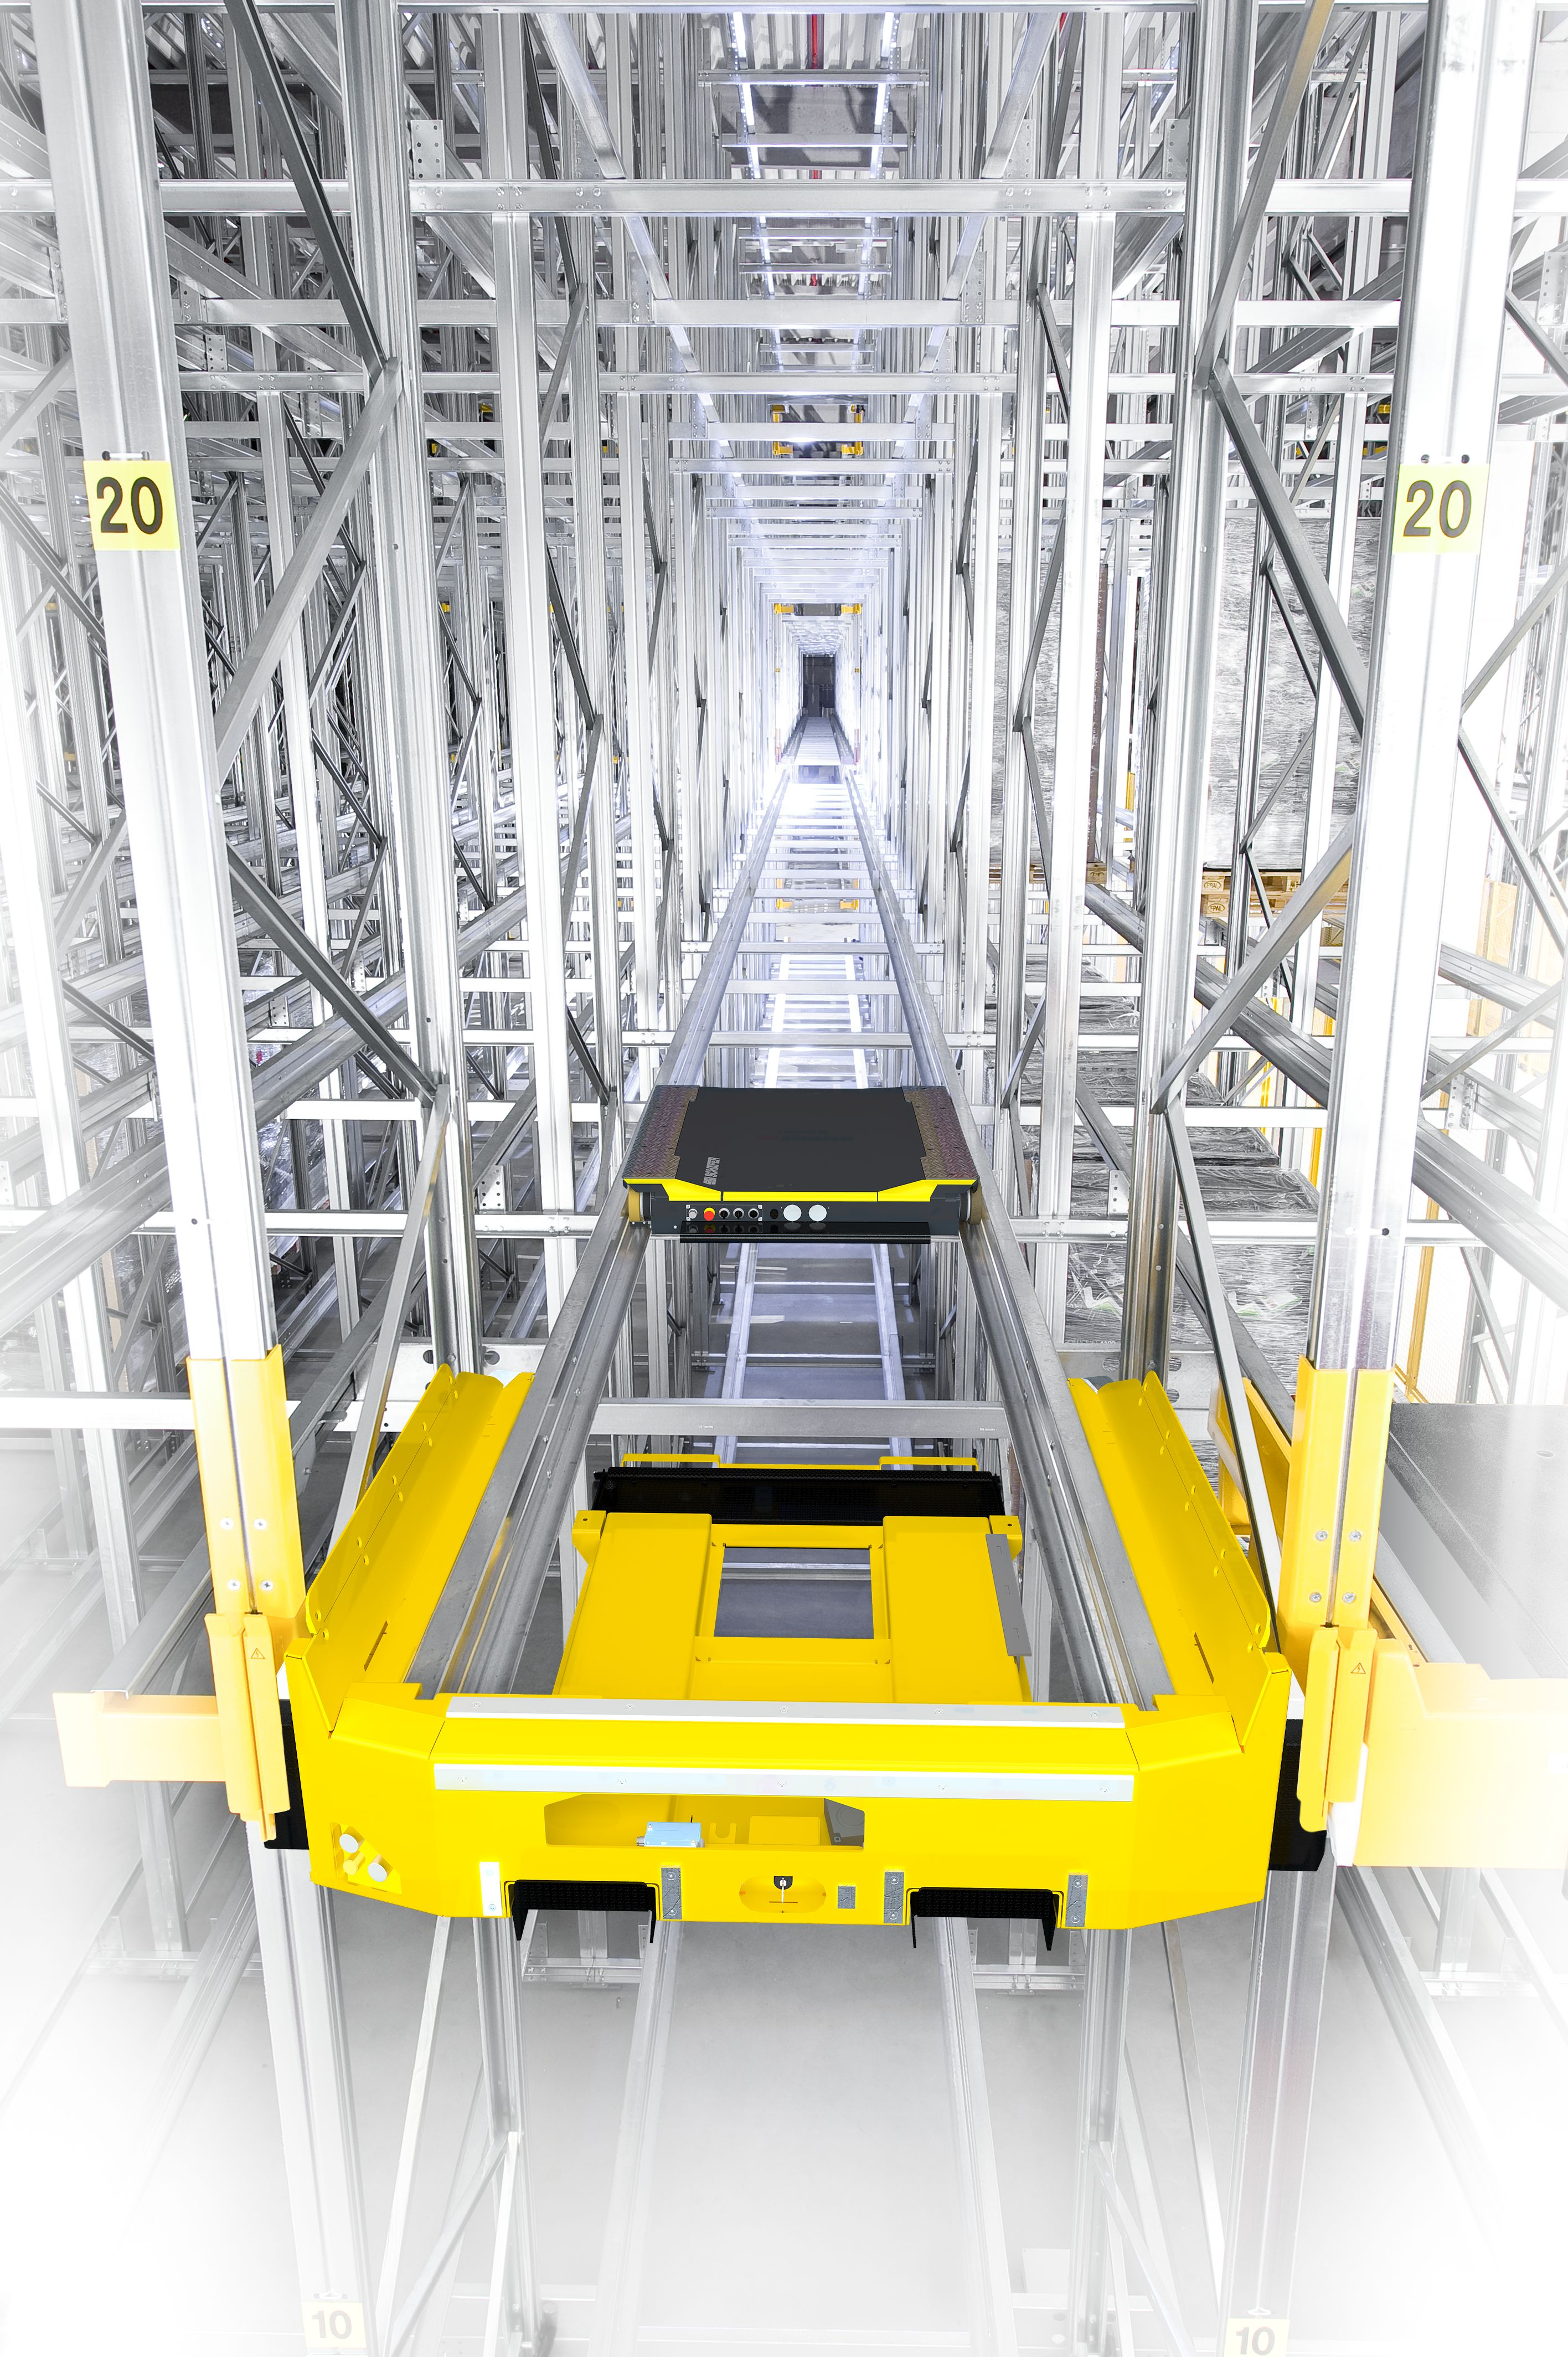
\includegraphics[width=\paperwidth,height=\paperheight]{images/ssi_orbiter_highlight.jpg}};

			%\vspace*{1cm}

			\Huge
			\textbf{Rapport de stage}

			\vspace{0.5cm}
			\LARGE
			"Développement Android"

			\vspace{1.5cm}

			\textbf{Anthony PINEAU}\\
			\textbf{IR2023}

			\vfill

			
\includegraphics[width=0.6\textwidth]{images/schaefer.jpg}
			\vfill
			
\includegraphics[width=0.4\textwidth]{images/esaip.jpg}

			\vfill

			Stage effectué du\\
			4 juillet 2022 au 26 août 2022

			\vspace{0.8cm}
			
			\Large
			Maître de stage : Monsieur Thierry NEROT\\
			Tuteur pédagogique : Monsieur Mathieu LAMBERT\\
		\end{center}
	\end{titlepage}
		
	\newpage

	\section*{Remerciements}		
	En premier lieu, je tiens à remercier Monsieur Laurent GOURDON, directeur général France de l'entreprise SSI SCHÄFER, de m’avoir permis de rejoindre son équipe et m’avoir offert la possibilité de mettre en pratique mes connaissances et mes compétences acquises pendant mes précédentes années d’études ainsi que ces deux premières années du cycle ingénieur du numérique à l’ESAIP. \\

	Je tiens ensuite à remercier Monsieur Thierry NEROT, qui, en tant que maître de stage, s'est rendu disponible pour moi, a su m'accompagner et partager ses connaissances.\\

	J’en profite pour remercier aussi tous les membres de l’équipe avec qui j’ai pu travailler, Messieurs Sébastien NICOD, Laurent BOURREAU, Thibaut LUCAS et Pascal MARCELOT, qui ont su se rendre disponible pour moi si besoin. Il a d'ailleurs été très facile pour moi de pouvoir échanger avec eux et j'ai beaucoup appris auprès d'eux.\\

	Par ailleurs, je remercie également tous mes autres collègues qui ont été très accueillants tout au long du stage, Mesdames Charlotte BARGMAN, Océane SACHOT, Pauline CHAPRON, Anita BABONNEAU, Nathalie DELARUE, Roukia ATHOUMANI ainsi que Messieurs Quentin VIOLLEAU, Robin BALLON et Nicolas PERDRIAU.\\

	Je saisis cette occasion pour adresser mes profonds remerciements aux responsables et au personnel de l’ESAIP d’avoir fait le nécessaire en ce qui concerne la gestion des conventions de stage ainsi que de nous soutenir au quotidien dans notre projet pédagogique et professionnel.\\

	Je tiens ainsi à remercier tout particulièrement Monsieur Mathieu LAMBERT. En tant que tuteur pédagogique, nous avons pu échanger lors d'une réunion en visioconférence au milieu de mon stage, et parler de l’avancement du projet sur lequel j'ai travaillé.\\

	Enfin un grand merci à ma famille, sans qui tout cela ne serait pas possible. Merci pour leurs conseils ainsi que leur soutien inconditionnel, à la fois moral et économique. Ils m’accompagnent et me soutiennent au quotidien aussi bien dans mon projet pédagogique que dans mon projet professionnel et sont une source d’inspiration pour moi.

	\newpage

	\section*{Mots clés}
	Liste des mots clés : android, développement, développement informatique, logistique, France, Cholet, WMS, WCS, socket, MORPHEUS, android studio, windev mobile.

	\newpage
	
	\doublespacing
	\tableofcontents

	\newpage
		
	\rfoot{Page \thepage}
	
	\phantomsection
	\listoffigures
	\addcontentsline{toc}{section}{\listfigurename}
			
	%\newpage

	%\phantomsection
	%\listoftables
	%\addcontentsline{toc}{section}{\listtablename}
	
	\newpage

	\phantomsection
	\printglossary
	\addcontentsline{toc}{section}{\glossaryname}

	\newpage
	
	\singlespacing

	\phantomsection
	\section*{Introduction}
	\addcontentsline{toc}{section}{Introduction}
%Introduire via la logistiqe..
	Des livraisons qui doivent être faites le jour même, adaptées aux magasins, un approvisionnement efficace de la production, ces exigences ne peuvent être satisfaites qu'à travers des produits et des processus logistiques efficaces. Ainsi dans le cadre de ma deuxième année de cycle ingénieur au sein de l’ESAIP, j’ai pu effectuer un stage, du 4 juillet 2022 au 26 août 2022, au sein de l’entreprise SSI SCHÄFER, dirigé, au niveau France, par Monsieur Laurent GOURDON.\\
%début inspiré de https://www.ssi-schaefer.com/fr-fr/produits

	L'entreprise SSI SCHÄFER est aujourd'hui l'un des premiers fournisseurs mondiaux de produits et systèmes logistiques pour le stockage, la préparation des commandes et la gestion des déchets. Ces solutions intralogistiques, partiellement ou entièrement automatisées, permettent d’optimiser les flux logistiques et l’aménagement des entrepôts et centres logistiques des clients, peu importe leur surface de stockage et leur secteur d’activité.\footnote{\cite{schaefer}}\\

%mission
	Ma mission pour ce stage a été d'évaluer et de comparer deux outils de développement d'une application Android pour le domaine industriel et logistique. En effet, j'ai eu l'opportunité de développer une copie de l'application android existante, développée sous windev mobile, qui permet d'utiliser le client morpheus sur des terminaux mobiles, en utilisant l'outil de développement Android Studio. Au-delà d'enrichir mes connaissances dans le domaine du développement android, ce stage m'a permis de découvrir un nouveau domaine pour moi, la logistique.\\

%plan
	En vue de rendre compte des deux mois passés dans la société SSI Schäfer, il apparaît important de poser le contexte global dans lequel s'est déroulé mon stage (entreprise d'accueil : SSI Schäfer, organisation...). Ainsi, nous pourrons déterminer mon positionnement en tant que stagiaire au sein de la structure. Nous aborderons ensuite le cahier des charges qui a été émis pour le projet qui m'a été donné. Puis nous parlerons de la méthodologie et des outils que j'ai utilisé et montrerons les résultats du projet. Nous ferons ensuite un bilan et une analyse du stage avant de finir avec une conclusion. Enfin, nous trouverons la bibliographie, l'index, les annexes ainsi qu'un résume du rapport en français, en anglais et en allemand.
	
	\newpage

	%glossaire
	%\gls{latex}
	%\Glspl{formula} première lettre majuscule et pluriel
	
	%acronyme
	%\acrlong{wms}
	%\acrshort{wms}
	%\acrfull{wms}
	
	%index
	%\index{maths}

	%index + glossaire..
	%\index{\gls{WMS}}

	%à voir index + glossaire + acronyme ..

	%bibliographie
	%\cite{ctan}
	\section{Contexte global\footnote{Références utilisées dans la section \ref{section:context} : \cite{schaefer}, \cite{history}, \cite{schaeferFR}, \cite{schaeferMorpheus}.}}\label{section:context}
		%introduction contexte global
	Afin de bien comprendre les intérêts de ce stage, il est important d'en poser le contexte et notamment de revenir sur l'entreprise SSI SCHÄFER ainsi que la suite de logiciels MORPHEUS.
	
		\subsection{L'entreprise : SSI SCHÄFER}
	L'entreprise SSI SCHÄFER est aujourd'hui l'un des premiers fournisseurs mondiaux de produits et systèmes logistiques pour le stockage, la préparation des commandes et la gestion des déchets. Ces solutions intralogistiques, partiellement ou entièrement automatisées, permettent d’optimiser les flux logistiques et l’aménagement des entrepôts et centres logistiques de nos clients, peu importe leur surface de stockage et leur secteur d’activité.

			\begin{figure}[h!]
				\begin{center}
					
\includegraphics[width=0.7\linewidth]{images/schaefer.jpg}
				\end{center}
				\caption{Logo de l'entreprise SSI SCHÄFER}
				\label{fig:schaefer}
			\end{figure}	
		
			\subsubsection{Histoire}
	C'est en 1935 que Fritz SCHÄFER (1893-1951) commença à construire ses premiers conteneurs de transport, pendant son temps libre, dans l'espace minuscule de sa propre buanderie. Deux ans plus tard, le plombier et soudeur de formation réalise son rêve et fonde son entreprise pour produire des « produits et articles en tôle ». L'entreprise a été officiellement enregistrée à Burbach, en Allemagne, le 16 janvier 1937. Elle connaît un succès immédiat et doit dès 1939 construire son premier grand hall de production.\\

	La société s'internationalise au début des années 1960 avec la création de filiale en Suisse et en Angleterre. En 1965, Fritz SCHÄFER commence désormais la production de rayonnages à étagères et à palettes. L'entreprise se diversifie à l'aube du deuxième millénaire avec la création de SSI SCHÄFER Noell et SSI SCHÄFER Peem qui proposent des prestations avec des solutions d'automatisation. C'est en 2005 que les trois entreprises se regroupent sous la marque SSI SCHÄFER.\\

				\begin{wrapfigure}{r}{0.5\textwidth}
					\label{fig:lager}
					\vspace{-20pt}
					\begin{center}
						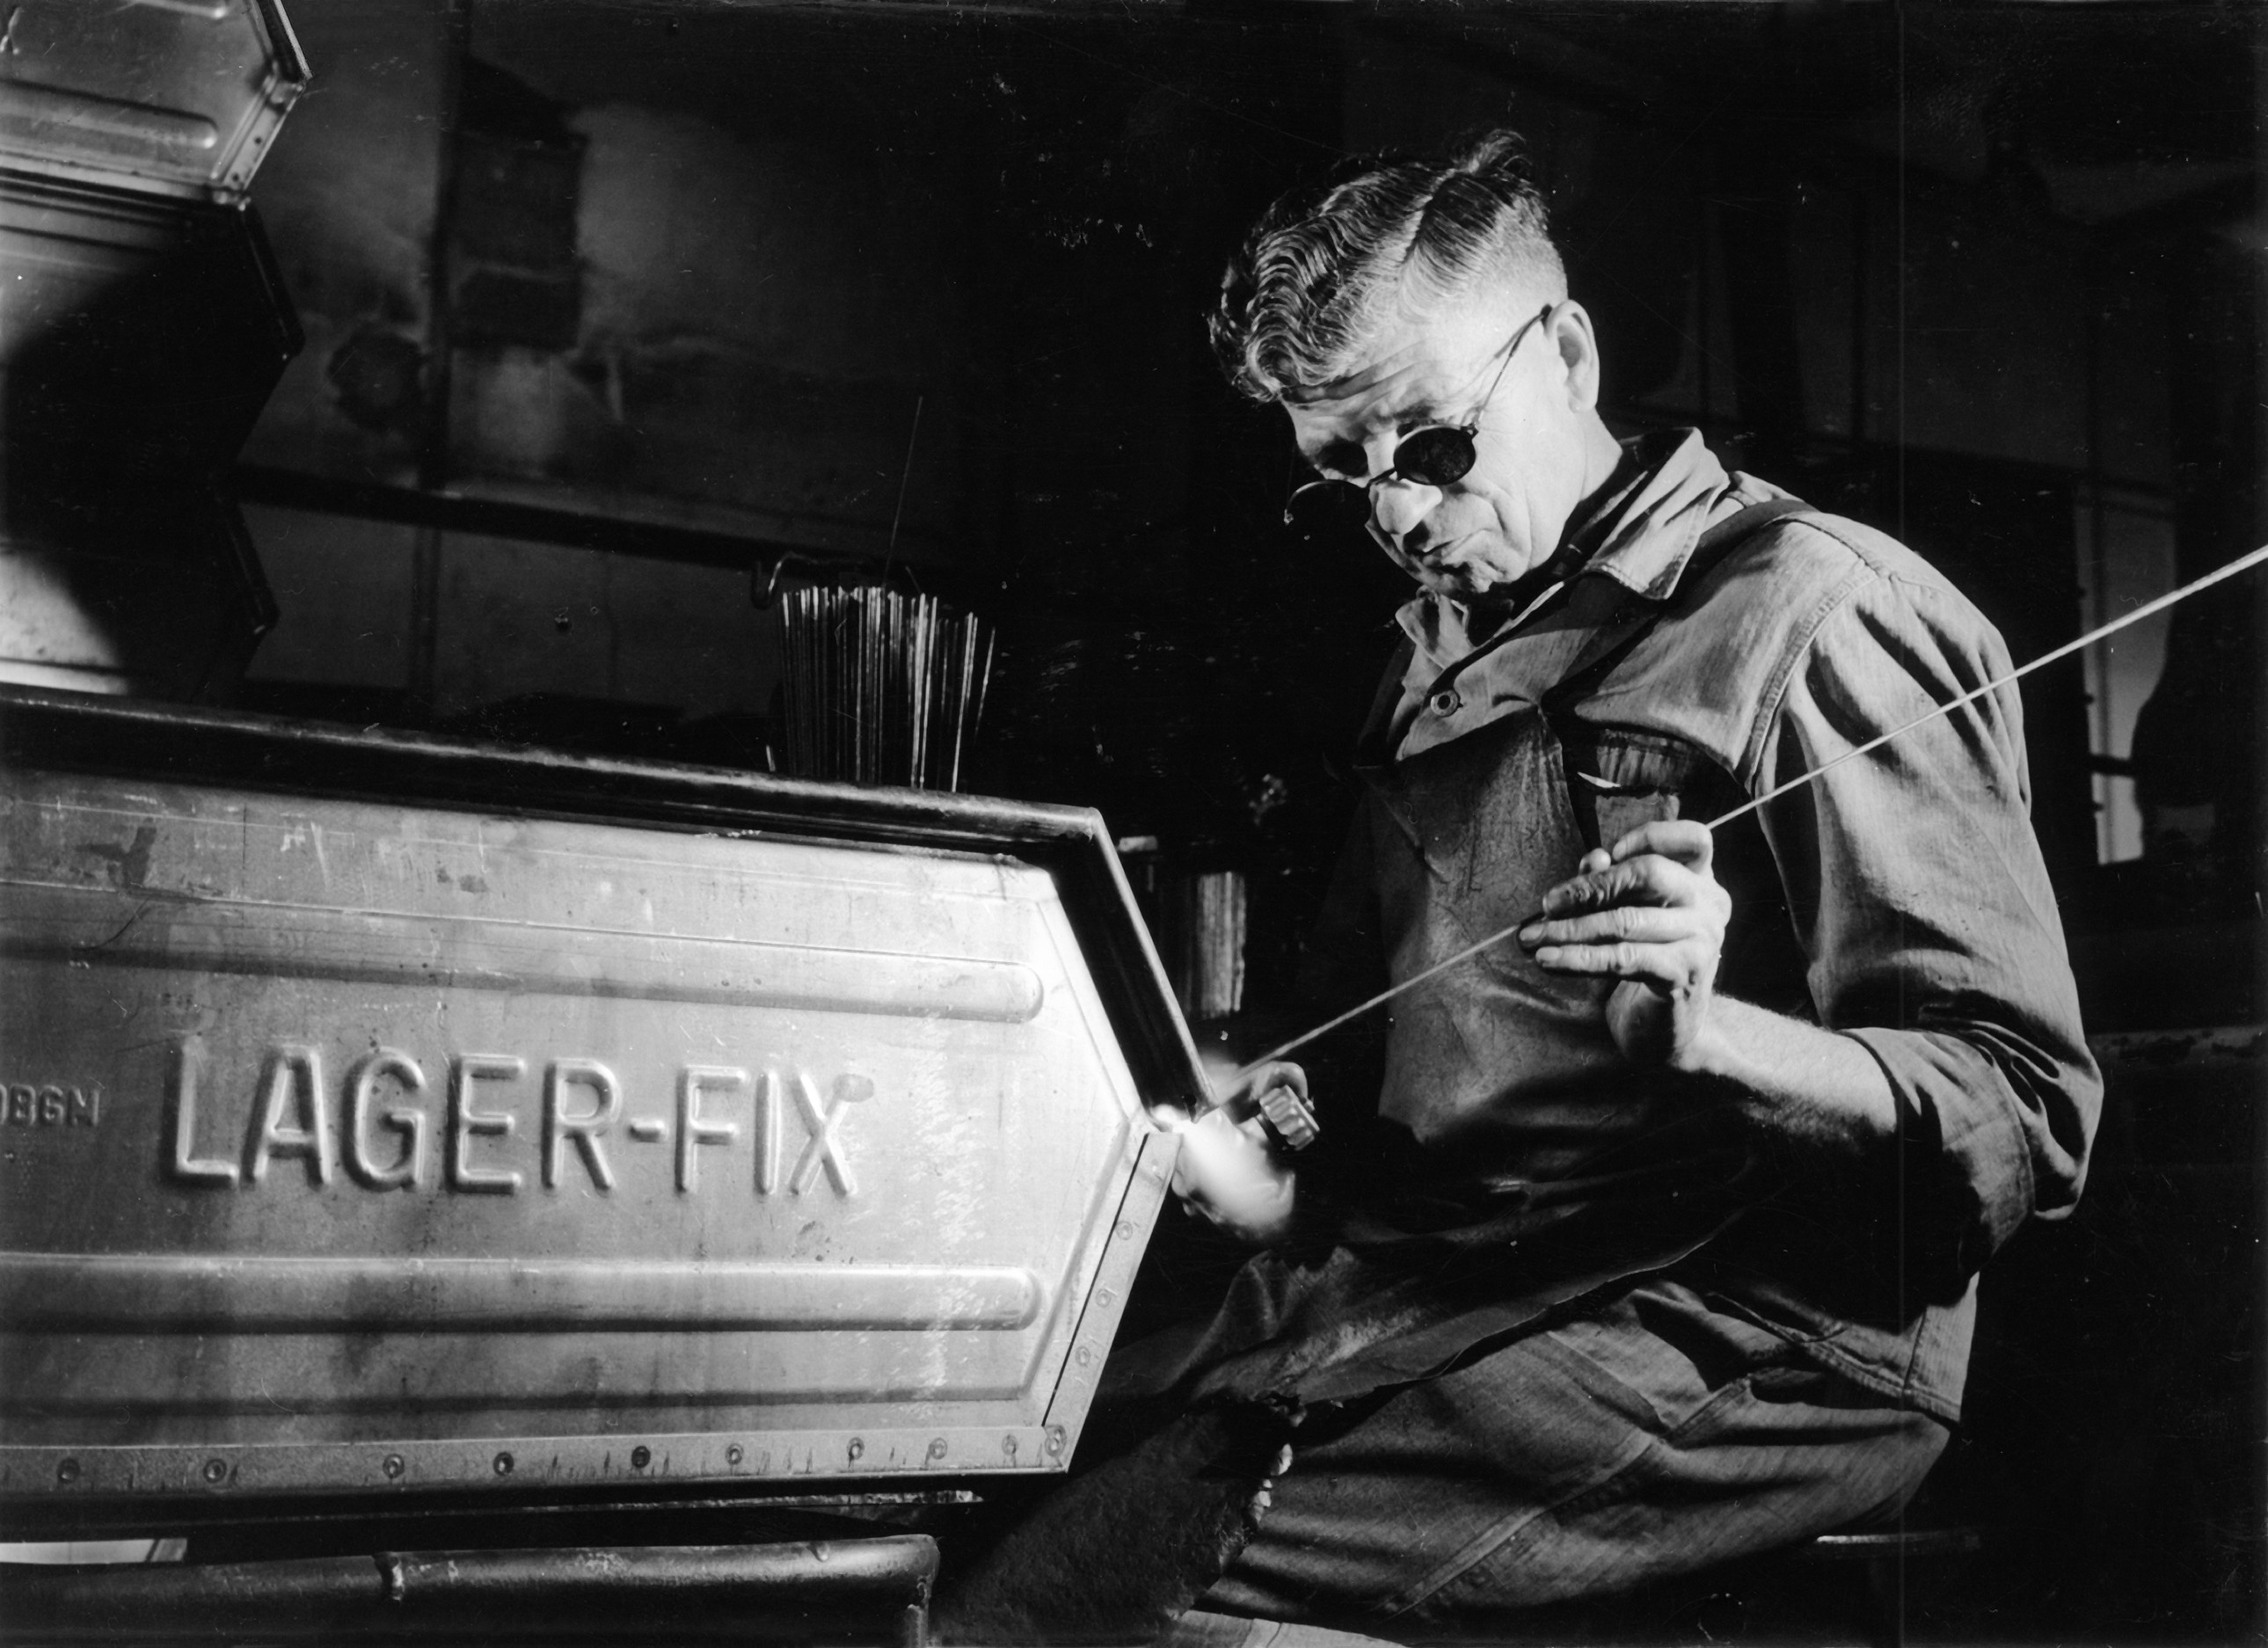
\includegraphics[width=0.48\textwidth]{images/lager_fix.jpg}
					\end{center}
					\vspace{-20pt}
					\caption{Lager fix}
					\vspace{-10pt}
				\end{wrapfigure}

	En 2008, le spécialiste logiciel, Salomon Automation, rejoint l'entreprise. Puis SSI SCHÄFER rachète l'entreprise danoise Handler A/S, expert en tours de stockage, en 2010. 2017 est un nouveau tournant pour l'entreprise avec la création de SSI SCHÄFER IT SOLUTIONS GMBH et une nouvelle dénomination sociale SSI SCHÄFER AUTOMATION GMBH.\\
			
	Vous pourrez par ailleurs trouver en annexe \ref{appendix:history} et \ref{appendix:map} une frise historique avec les dates importantes de l'histoire SSI SCHÄFER ainsi que la carte de toutes les filiales de l'entreprise.

			\subsubsection{SSI SCHÄFER en France}
	Le groupe SSI SCHÄFER est représenté par deux filiales en France, qui couvrent l'ensemble du territoire français et des besoins intralogistiques.\\

	Créée en 1963, SSI SCHAEFER SAS a son siège en historique en Moselle, on y retrouve notamment toutes les fonctions administratives et de soutien stratégique ainsi que la conception. Les commerciaux et techniciens de maintenance sont déployés sur l'ensemble du territoire français, ce qui garantit une proximité avec les clients et des temps de réaction brefs dans toute la France.\\

	En automne 2017, SSI SCHÄFER fait l'acquisition de GRN Logistic, basé à Cholet, qui vient compléter, de par son expertise dans le domaine des logiciels logistiques, l'expérience nationale et internationale du groupe dans la vente de solutions intralogistiques. Ce qui vient améliorer la compétence globale de SSI SCHÄFER en France.
			
		\subsubsection{Solutions intralogistiques}
	SSI SCHÄFER élabore, conçoit et fabrique des systèmes intralogistiques modulaires, destinés à tous les besoins en stockage, préparation de commandes et convoyage :
				\begin{itemize}
					\bdot{Solutions de stockage}
						\begin{itemize}
							\bdotoutlined{Rayonnage tous types}
							\bdotoutlined{Bacs et conteneurs}
							\bdotoutlined{Tours de stockage}
							\bdotoutlined{Transstockeurs}
							\bdotoutlined{Navettes}
							\bdotoutlined{Orbiters}
						\end{itemize}
					\bdot{Solutions de convoyage}
						\begin{itemize}
							\bdotoutlined{Convoyeur de bacs, cartons, palettes et plateaux}
							\bdotoutlined{Convoyeur aérien}
							\bdotoutlined{Système de transport sans conducteurs (AGVs)}
						\end{itemize}
					\bdot{Systèmes de préparation de commandes}
						\begin{itemize}
							\bdotoutlined{"Man to products" : pick by light, pick by voice, RF picking}
							\bdotoutlined{"Products to Man": caroussel, trieur, A-Frame, pick to tote}
							\bdotoutlined{Tours de stockage et rayonnages dynamiques}
						\end{itemize}
					\bdot{Solutions clefs en main}
						\begin{itemize}
							\bdotoutlined{Planification logistique globale et conseil}
							\bdotoutlined{Construction des bâtiments et installations}
							\bdotoutlined{Prestations de service et de maintenance sur mesure}
						\end{itemize}
				\end{itemize}

			\begin{figure}[h!]
				\begin{center}
					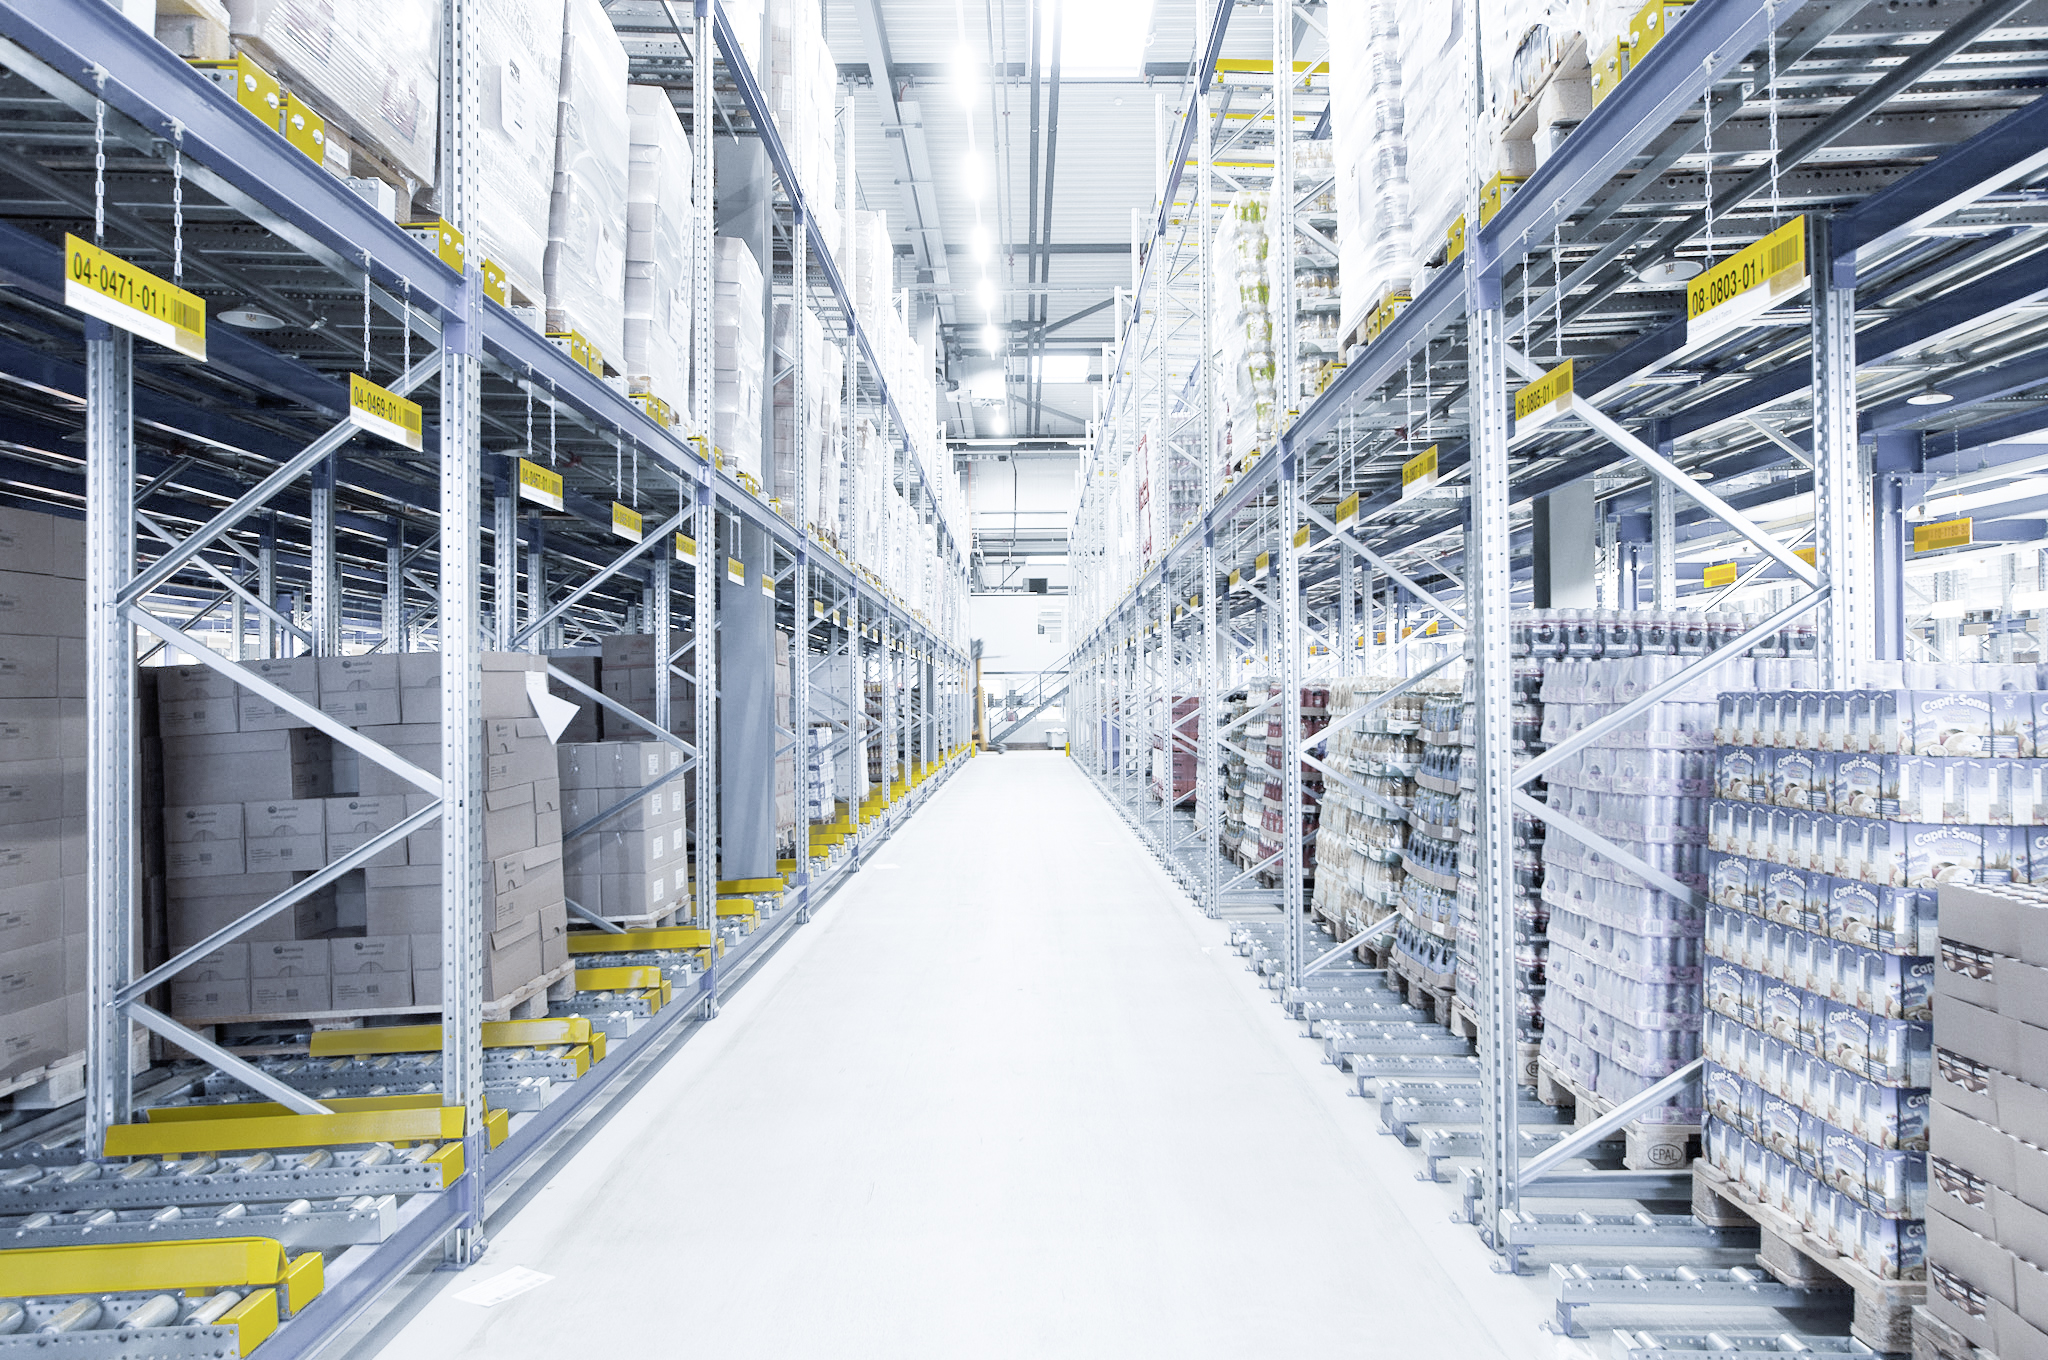
\includegraphics[width=0.7\linewidth]{images/intralogistic.jpg}
				\end{center}
				\caption{Exemple de solution intralogistique}
				\label{fig:intralogistic}
			\end{figure}	
	
			\subsubsection{Solutions logicielles}
	Les processus intralogistiques sont de plus en plus complexes. Dans les entrepôts manuels, automatisés et entièrement automatisés, d'innombrables processus doivent être contrôlés, visualisés et optimisés. Cela exige de l'expertise. En tant que premier fournisseur mondial de systèmes logistiques, SSI SCHÄFER ne se contente pas de proposer tout ce dont on a besoin pour des entrepôts, mais propose également l'expertise informatique.\\

				\noindent
				Exemples de logiciels logistiques développés par SSI SCHÄFER :
				\begin{itemize}
					\bdot{WAMAS}
					\bdot{MORPHEUS}
				\end{itemize}
				\vspace{\baselineskip}
				\par Nous nous intéresserons ici à MORPHEUS, logiciel développé en France par GRN Logistics, avec lequel j'ai travaillé durant mon stage.
		\subsection{MORPHEUS}
	La suite logicielle MORPHEUS est une gamme de logiciels dédiée à la gestion et à l'optimisation de la performance de la logistique. Elle est composée de différents modules :
			\begin{itemize}
				\bdot{\index{\gls{WMS}} (Gestion des entrepôts)}
				\bdot{\index{\gls{WCS}} (Pilotage de stockeurs et de préparation de commandes automatisés}
			\end{itemize}
			\subsubsection{Morpheus \acrshort{wms}}
				\noindent				
				Les objectifs du WMS :
				\begin{itemize}
					\bdot{Augmenter votre productivité}
					\bdot{Réduire les stocks}
					\bdot{Optimiser les surfaces de stockages}
					\bdot{Diminuer les erreurs}
				\end{itemize}
				\vspace{\baselineskip}
				Quelques fonctionnalités du WMS :
				\begin{itemize}
					\bdot{Moteur de règles pour la gestion des stratégies métiers}
					\bdot{Planification et pré-réception}
					\bdot{Création et affectation automatique des emplacements}
					\bdot{Ordonnancement manuel et automatique}
					\bdot{Pilotage des ressources humaines}
				\end{itemize}
				%WMS Annexe \ref{appendix:morpheusWMSFonctionnalites}
				%cf annexe fonctionnalités morpheus WMS
			\subsubsection{Morpheus \acrshort{wcs}}
				\noindent
				Les objectifs du WCS :
				\begin{itemize}
					\bdot{Mécaniser et automatiser les flux}
					\bdot{Intégrer et synchroniser les WMS \& WCS}
					\bdot{Séquencez l'activité des équipements}
					\bdot{Superviser et optimiser les process}
				\end{itemize}
				\vspace{\baselineskip}
				Quelques fonctionnalités du WCS :
				\begin{itemize}
					\bdot{Pilotage de covoyeurs pour le transport de cartons, bacs...}
					\bdot{Pilotage du stockage et de la prépartion de commandes}
					\bdot{Pilotage des trieurs / robots / meubles de tri}
				\end{itemize}
				\vspace{\baselineskip}
			%cf annexe fonctionnalités morpheus WCS
			%mettre toutes les fonctionnalités en annexe ..
			Retrouvez plus d'informations sur le WMS et le WCS en annexe \ref{appendix:morpheusWMSFonctionnalites} et \ref{appendix:morpheusWCSFonctionnalites}

			\subsubsection{Application existante}
	À l'heure actuelle, la plupart des terminaux utilisés dans les entrepôts logistiques sont sous Windows CE, une application avait donc été développée pour communiquer avec la base de données utilisée par MORPHEUS. Néanmoins, comme les technologies évoluent, les terminaux commencent peu à peu à passer sous système android, ainsi une application a été developpée sous Windev Mobile pour être utilisée sous Android.
%				parler de l'application pour windows CE
%				puis migration sur android donc nouvelle application, première sous windev et voulu tester android studio..

		\subsection{Organisation}
	Pour ce stage, mes horaires de travail étaient 8 h 30 - 12 h 30 et 13 h 30 - 16 h 30 du lundi au vendredi. J'ai principalement travaillé en autonomie, néanmoins, je pouvais demander de l'aide à mes collègues dès que j'en avais besoin. Par ailleurs, nous faisions une réunion tous les vendredis à 14 h avec tous les développeurs où chacun disait ce qu'il avait fait dans la semaine et pouvait montrer son travail, c'était le "Point Dev". Dans la journée, je laissais toujours Teams ainsi qu'Outlook ouvert pour pouvoir interagir avec les collègues en télétravail.\\

	\newpage

	\section{Positionnement du stagiaire}
		Mon stage a débuté le lundi 4 juillet 2022, à cette occasion, j'ai pu rejoindre le service informatique de l'entreprise et découvrir plus en détail la mission qui allait m'être confiée durant les deux prochains mois. J'ai ainsi intégré le service informatique en tant que stagiaire développeur et rejoint l'équipe de développeurs, composée de Messieurs Sébastien NICOD, Laurent BOURREAU, Thibaut LUCAS et Pascal MARCELOT sous la supervision de Monsieur Thierry NEROT.
		\subsection{Mission}
	L'objectif de ce stage est d'évaluer et de comparer deux outils de développement d'une application Android pour le domaine industriel et logistique. Ainsi, la mission qui m'a été proposée, a été de réaliser un comparatif technique entre la solution actuelle de l'entreprise, Windev Mobile, et l'éditeur de code Android Studio.\\

	\noindent
	Les intérêt du projet pour l'entreprise sont :
		\begin{itemize}
			\bdot{Veille technologique}
			\bdot{Remise en cause éventuel de l'outil de développement actuellement utilisé}
			\bdot{Échanges avec les équipes}
		\end{itemize}
	
	\vspace{\baselineskip}
	\noindent
	Le comparatif technique entre les deux solutions portera sur les points suivants :
		\begin{itemize}
			\bdot{Environnement de développement}
			\bdot{Facilité d'utilisation}
			\bdot{Temps de développement}
			\bdot{Fonctionnalités}
			\bdot{Robustesse}
			\bdot{outils de simulation et de test}
			\bdot{Suivi des mises à jour Android et migrations}
			\bdot{Déploiement final}
		\end{itemize}
	
		\vspace{\baselineskip}
		\par L'objectif de l'application est de pouvoir se connecter, à travers un serveur socket, à la base de données utilisée par le logiciel MORPHEUS WMS.
		L'objectif final de ce stage sera donc de présenter une conclusion finale de préconisation de l'outil le plus adapté aux besoins de l'entreprise.
		%de faire une application de test sous Android Studio connecté à notre logiciel MORPHEUS WMS
		%de présenter une conclusion finale de préconisation de l'outil le plus adapté à notre besoin
	
	\newpage

	\section{Cahier des charges}
		L'objectif premier de ce stage était de réaliser un comparatif entre les deux outils de développement : Windev Mobile et Android Studio. Afin de réaliser au mieux cette comparaison, il m'est apparu logique d'essayer de reproduire l'application développée avec Windev Mobile et de la coder sous Android Studio.\\

		Afin de m'aider dans la conception de l'application, il m'a été fourni une liste des fenêtres à implémenter avec leurs caractéristiques dont voici la liste :
		\begin{itemize}
			\bdot{Fenêtre main}
				\begin{itemize}
					\bdotoutlined{Menu à gauche : menu application}
					\bdotoutlined{Menu à droite : menu utilisateur}
				\end{itemize}
			\bdot{Fenêtre Menu : Listes de bouons}
				\begin{itemize}
					\bdotoutlined{Choix de la disposition des boutons (nombre en largeur, nombre en hauteur)}
					\bdotoutlined{Choix de la couleur du bouton}
					\bdotoutlined{Choix de l'icône dans une bibliothèque}
					\bdotoutlined{Position de l'icône en fixe à gauche}
					\bdotoutlined{Libellé du bouton}
					\bdotoutlined{Choix de la fonction du bouton dans une liste}
				\end{itemize}
			\bdot{Fenêtre Login : Login, Matricule, Password (saisie et scan possible)}
			\bdot{Fenêtre Message}
				\begin{itemize}
					\bdotoutlined{Titre}
					\bdotoutlined{Couleur de fond}
					\bdotoutlined{Image jpeg}
					\bdotoutlined{X lignes dans un tableau}
					\bdotoutlined{Champs commentaire}
					\bdotoutlined{Liste des boutons}
					\bdotoutlined{Choix de la couleur du bouton}
					\bdotoutlined{Choix de l'icône dans une bibliothèque}
					\bdotoutlined{Position de l'icône en fixe à gauche}
					\bdotoutlined{Libellé du bouton}
					\bdotoutlined{Choix de la fonction du bouton dans une liste}
				\end{itemize}
			\bdot{Fenêtre saisie}
				\begin{itemize}
					\bdotoutlined{Titre}
					\bdotoutlined{Couleur de fond}
					\bdotoutlined{Image jpeg}
					\bdotoutlined{X lignes dans un tableau}
						\begin{itemize}
							\bsquare{Paramétrage}
							\bsquare{Longueur maximale}
							\bsquare{Type : numérique, numérique réel, alphanumériqué, date}
							\bsquare{Obligatoire : oui/non}
						\end{itemize}
					\bdotoutlined{Champs commentaire}
					\bdotoutlined{Liste des boutons}
					\bdotoutlined{Choix de la couleur du bouton}
					\bdotoutlined{Choix de l'icône dans une bibliothèque}
					\bdotoutlined{Position de l'icône en fixe à gauche}
					\bdotoutlined{Libellé du bouton}
					\bdotoutlined{Choix de la fonction du bouton dans une liste}
				\end{itemize}
			\bdot{Fenêtre Liste Tableau}
				\begin{itemize}
					\bdotoutlined{Titre}
					\bdotoutlined{Couleur de fond}
					\bdotoutlined{Image jpeg}
					\bdotoutlined{X lignes dans un tableau}
					\bdotoutlined{Liste des boutons}
					\bdotoutlined{Choix de la couleur du bouton}
					\bdotoutlined{Choix de l'icône dans une bibliothèque}
					\bdotoutlined{Position de l'icône en fixe à gauche}
					\bdotoutlined{Libellé du bouton}
					\bdotoutlined{Choix de la fonction du bouton dans une liste}
				\end{itemize}
			\bdot{Fenêtre Emplacement Détail}
				\begin{itemize}
					\bdotoutlined{Titre}
					\bdotoutlined{Couleur de fond}
					\bdotoutlined{Des onglets à faire défiler avec un glisser horizontal}
					\bdotoutlined{Liste des champs}
					\bdotoutlined{Graphique de l'emplacement}
					\bdotoutlined{Bouton OK}
					\bdotoutlined{Onglet 1 : Résumé}
					\bdotoutlined{Onglet 2 : Graphique}
					\bdotoutlined{Onglet 2 : Détail Emplacement}
					\bdotoutlined{Onglet 4 : Détail Article}
				\end{itemize}
			\bdot{Fenêtre Container Détail}
				\begin{itemize}
					\bdotoutlined{Titre}
					\bdotoutlined{Couleur de fond}
					\bdotoutlined{Des onglets à faire défiler avec un glisser horizontal}
					\bdotoutlined{Liste des champs}
					\bdotoutlined{Graphique du container}
					\bdotoutlined{Bouton OK}
					\bdotoutlined{Onglet 1 : Résumé}
					\bdotoutlined{Onglet 2 : Graphique}
					\bdotoutlined{Onglet 2 : Détail}
					\bdotoutlined{Onglet 4 : Tableau des supports}
				\end{itemize}
			\bdot{Fenêtre Article Détail}
				\begin{itemize}
					\bdotoutlined{Titre}
					\bdotoutlined{Couleur de fond}
					\bdotoutlined{Des onglets à faire défiler avec un glisser horizontal}
					\bdotoutlined{Liste des champs}
					\bdotoutlined{Photo}
					\bdotoutlined{Bouton OK}
					\bdotoutlined{Onglet 1 : Résumé}
					\bdotoutlined{Onglet 2 : Photo}
					\bdotoutlined{Onglet 2 : Détail}
					\bdotoutlined{Onglet 4 : Emplacements}
				\end{itemize}
			\bdot{Fenêtre Emplacement}
				\begin{itemize}
					\bdotoutlined{Titre}
					\bdotoutlined{Couleur de fond}
					\bdotoutlined{Des onglets à faire défiler avec un glisser horizontal}
					\bdotoutlined{Liste des champs}
					\bdotoutlined{Graphique de l'emplacement en 3D ou 2D}
					\bdotoutlined{Bouton OK}
					\bdotoutlined{Onglet 1 : Résumé}
					\bdotoutlined{Onglet 2 : Graphique}
					\bdotoutlined{Onglet 2 : Détail Emplacement}
					\bdotoutlined{Onglet 4 : Détail Article}
				\end{itemize}
			\bdot{Fenêtre Transaction}
				\begin{itemize}
					\bdotoutlined{Enchaînement des différentes transactions}
				\end{itemize}
			\bdot{Fenêtre Réception/Dépôtage}
				\begin{itemize}
					\bdotoutlined{Titre}
					\bdotoutlined{Couleur de fond}
					\bdotoutlined{Des onglets à faire défiler avec un glisser horizontal}
					\bdotoutlined{Liste des champs}
					\bdotoutlined{Graphique de l'emplacement}
					\bdotoutlined{Zone de scan}
					\bdotoutlined{Bouton OK}
				\end{itemize}
		\end{itemize}
		\vspace{\baselineskip}
		Néanmoins, ceci n'était pas un cahier des charges strict au sens du terme, en effet, j'ai été assez libre d'adapter certains designs. De plus, je n'avais pas de contraintes sur la partie fonctionnelle de l'application et j'ai donc pu mettre en œuvre la configuration qui me semblait la plus adéquat pour la connexion socket à la base de données. Ainsi, j'ai pu développer l'application en m'inspirant de l'application existante, développée par Monsieur Sébastien NICOD, en essayant d'implémenter les fenêtres de la liste que l'on m'a fourni et mes propres choix.
	\newpage

	\section{Méthodologie et outils}
		\subsection{Méthodologie}
			Ayant travaillé tout seul sur le projet, je n'ai pas vraiment suivi de méthodologie particulière. J'ai néanmoins travaillé étape par étape et ai fait progresser mon application petit à petit vers le résultat attendu. De plus, j'ai beaucoup fait de recherches sur Internet pour m'aider dans mon travail et demandé de l'ai à mes collègues quand j'en avais besoin. La documentation Android étant bien fournie j'ai aussi pu m'en servir assez régulièrement.
		\subsection{Outils}
		\noindent
		Voici la liste des outils que j'ai utilisé tout au long de mon projet :
		\begin{itemize}
			\bdot{Android Studio}
			\bdot{Word}
			\bdot{Latex}
			\bdot{Visual Studio Code}
			\bdot{Windev Mobile}
			\bdot{Microsoft SQL Server Management Studio}
			\bdot{Serveur socket (codé en interne) pour se connecter à la base de données}
			\bdot{Filezilla et Filezilla Server}
			\bdot{Google Chrome}
		\end{itemize}

	\newpage

	\section{Résultats}
		%résultats + screen application...		
		Ainsi après deux mois de travail voici le résultat de l'application que j'ai développé :\\
		%image activité d'accueil
		%mettre en annexe les autres screens

			\begin{figure}[h!]
				\begin{center}
					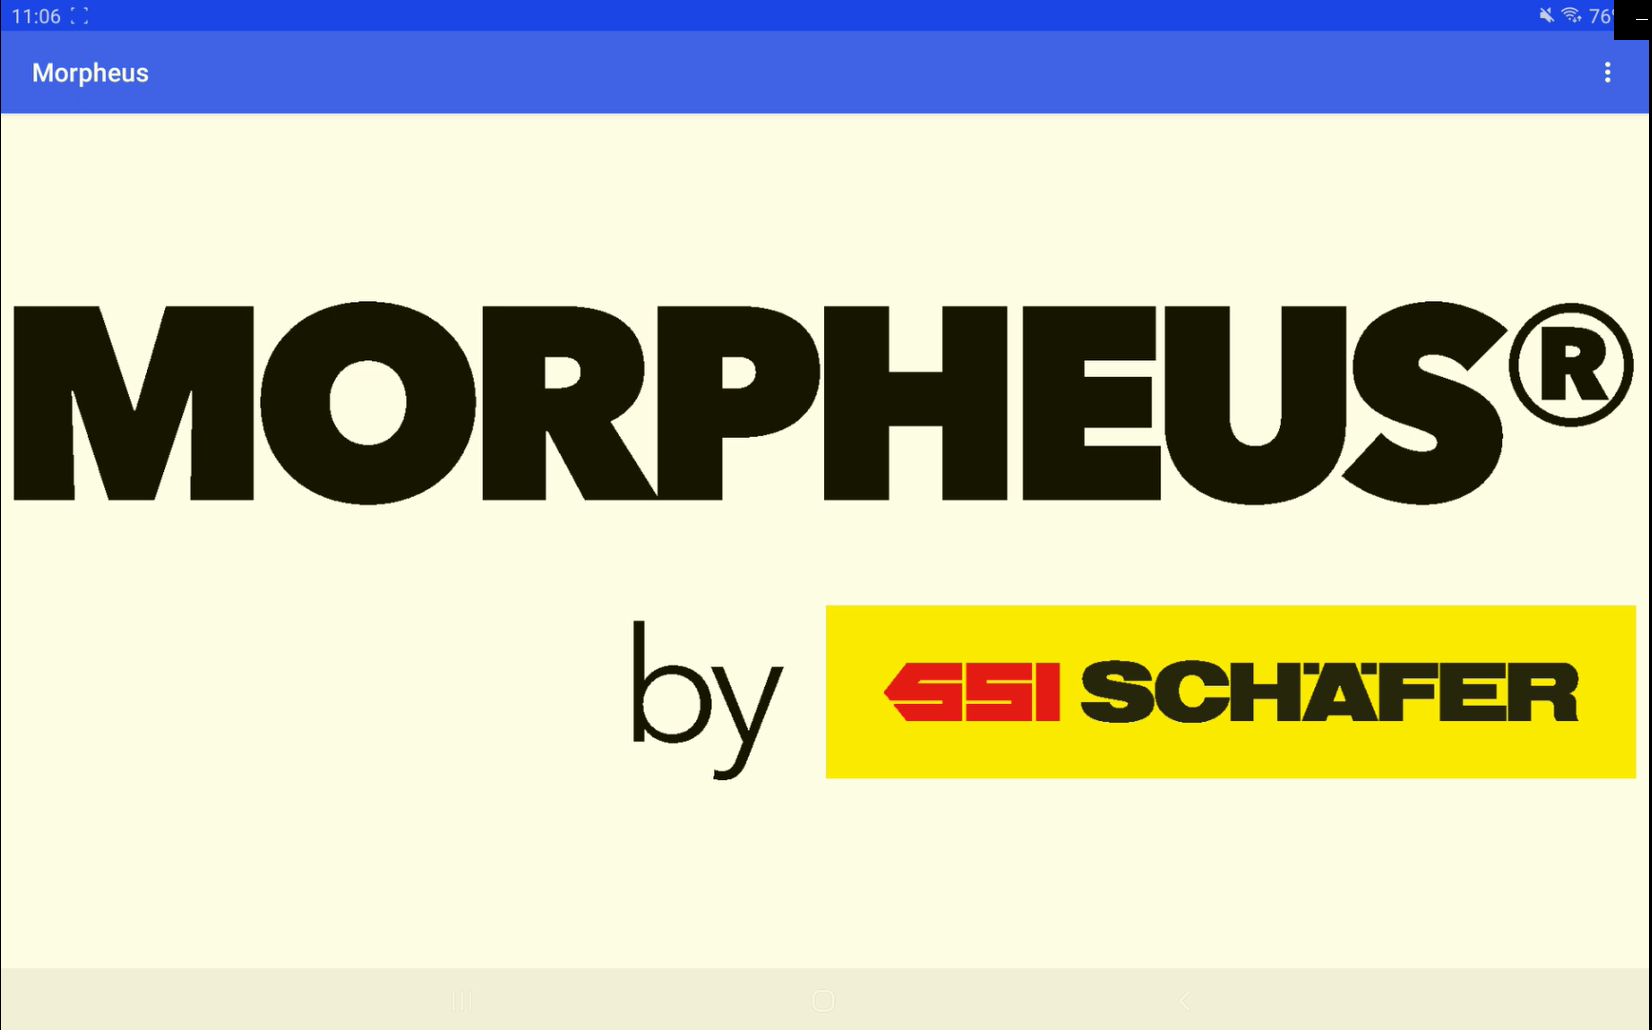
\includegraphics[width=0.7\linewidth]{application/main.PNG}
				\end{center}
				\caption{Écran d'accueil de l'application}
				\label{fig:applications:main}
			\end{figure}	

\vfill

			\begin{figure}[h!]
				\begin{center}
					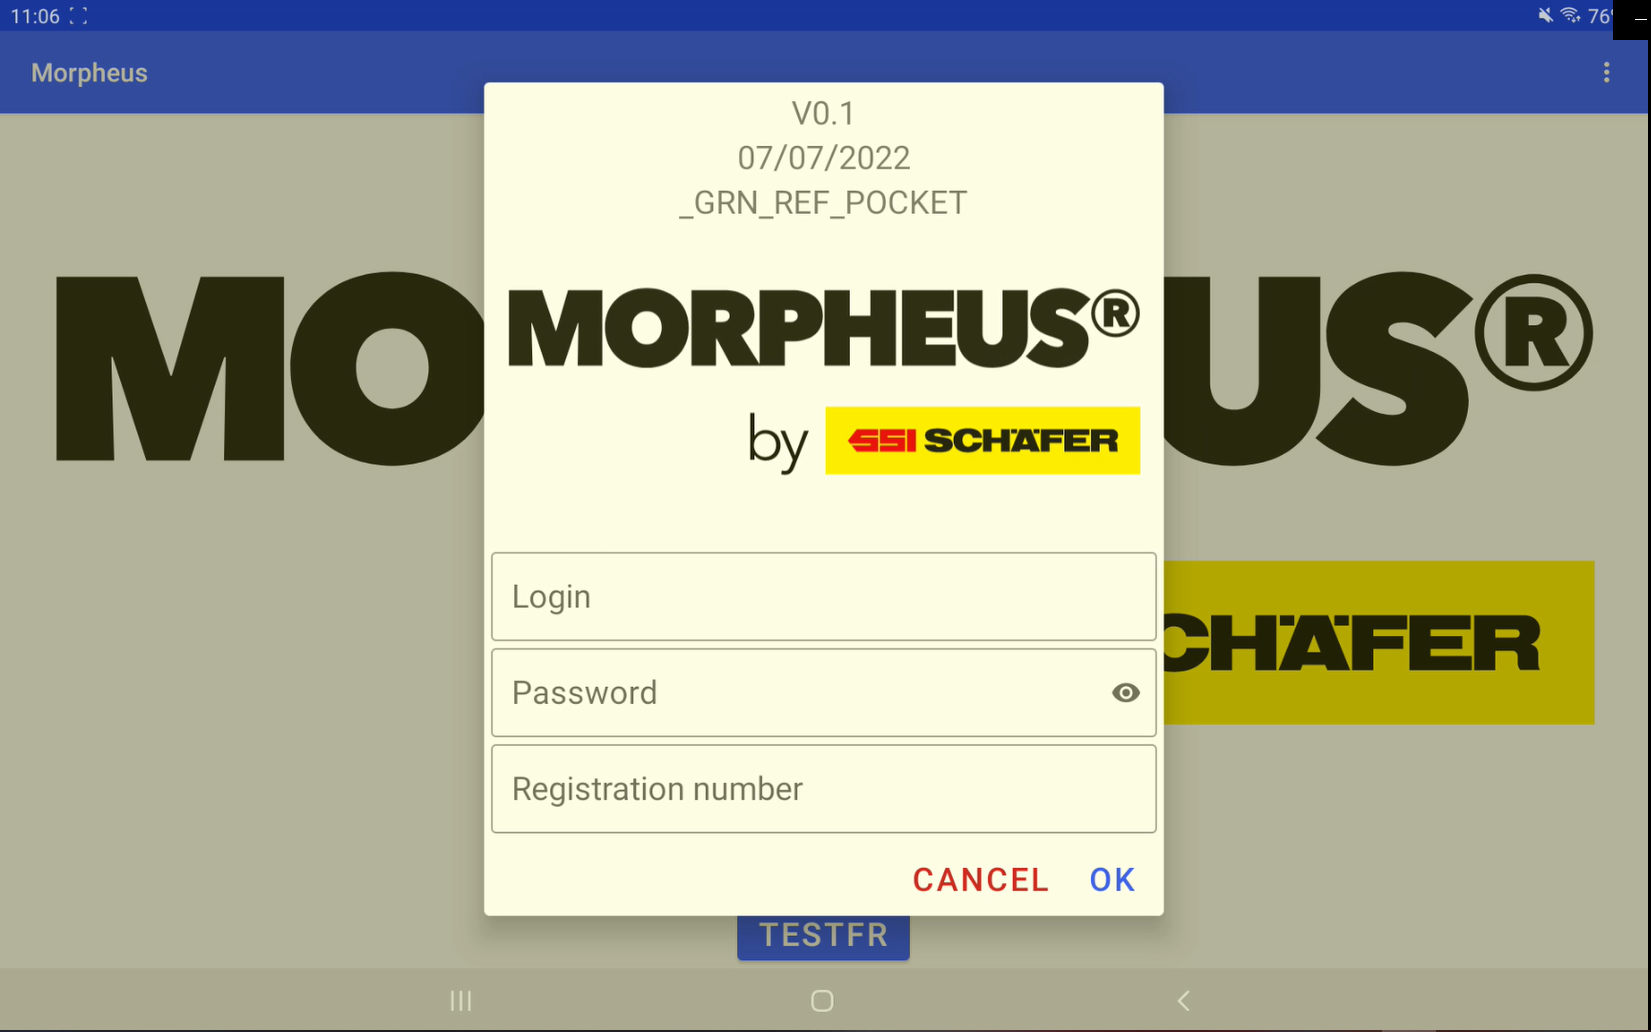
\includegraphics[width=0.7\linewidth]{application/login.PNG}
				\end{center}
				\caption{Écran de connexion de l'application}
				\label{fig:applications:login}
			\end{figure}	

\newpage

			\begin{figure}[h!]
				\begin{center}
					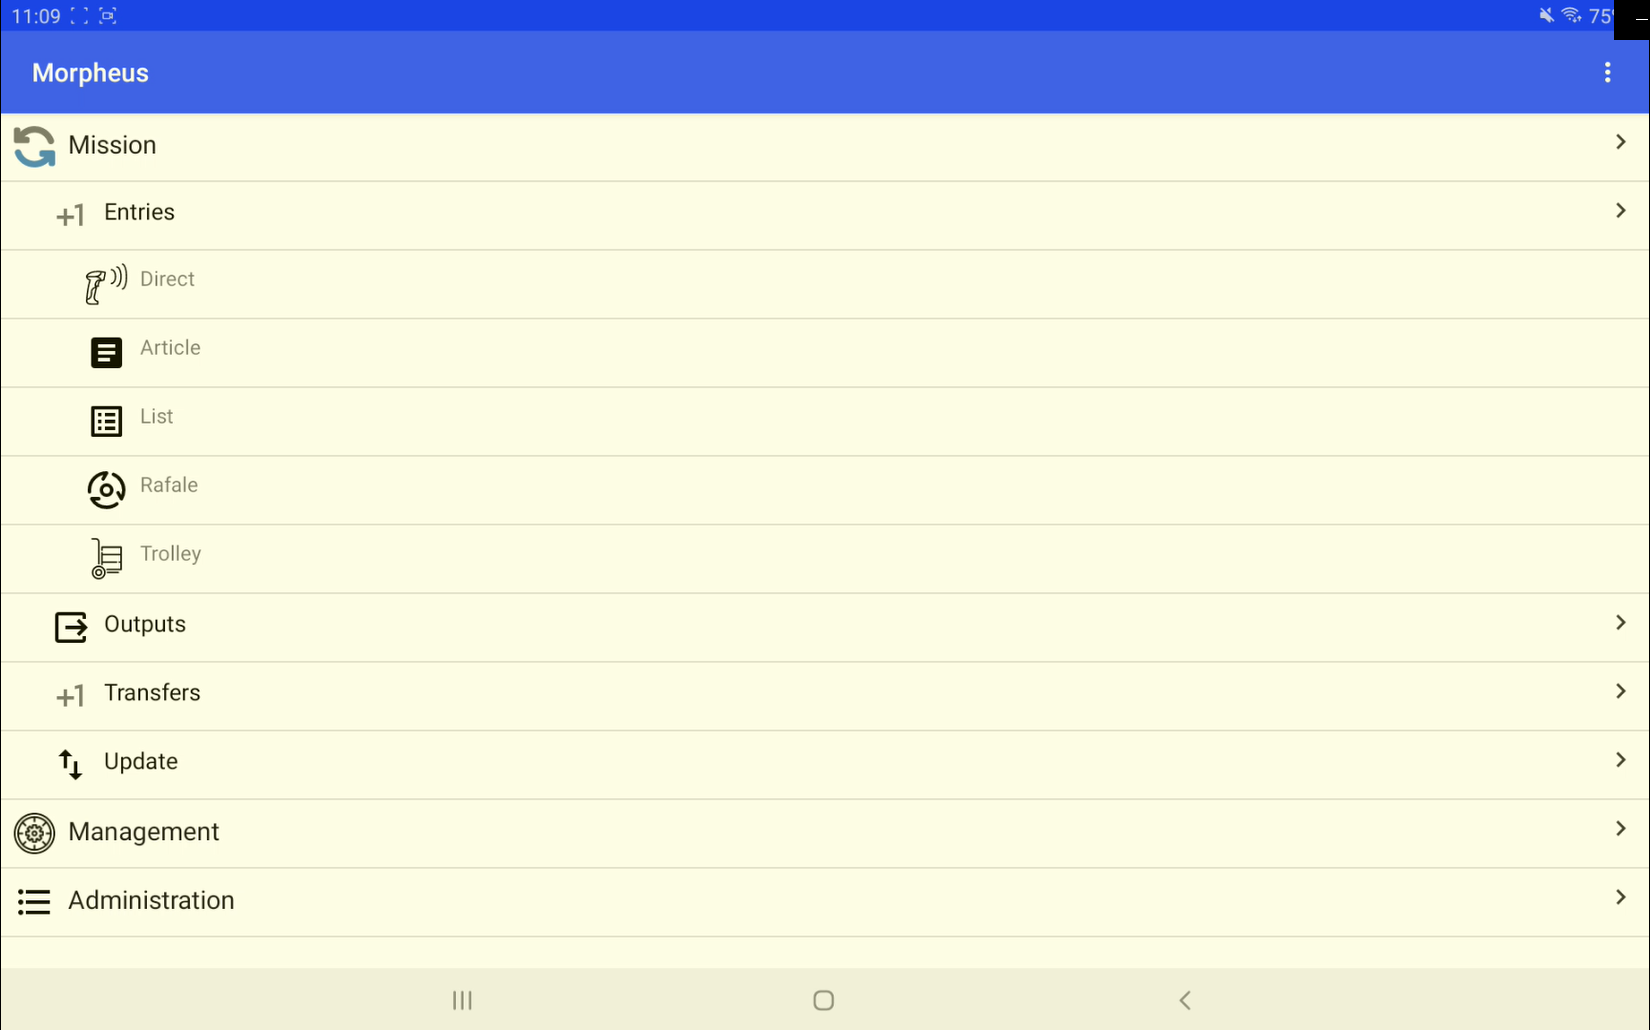
\includegraphics[width=0.7\linewidth]{application/user_menu_subtab.PNG}
				\end{center}
				\caption{Écran du menu utilisateur de l'application}
				\label{fig:applications:user_menu_subtab}
			\end{figure}

		Malheureusement, malgré le développement de cette application, je n'ai pas eu le temps de comparer les deux outils de développement sur tous les points de comparaison qui avaient été établis, néanmoins j'ai pu remarquer que les deux environnement étaient globalement équivalents, bien que le temps de développement sous Android soit légèrement plus rapide.	 Le choix de conserver Windev Mobile ou de passer sur Android Studio n'a pour le moment pas été fait.\\
		
		Vous trouverez toutes les autres captures d'écran de l'application en Annexe \ref{appendix:application}.
	
%		Le développement de cette application ne m'a malheuresement pas permis de comparer les deux outils de développement 
		%Le développement de cette application m'a donc permis de comparer les deux outils de développement.

		%\subsection{Comparaison entre les deux outils de développement}
			%tableau de comparaison
			%À la fin de ce projet, j'ai donc pu établir un petit comparatif des deux outils de développement, néanmoins, je n'ai pas pu traiter tous les points de comparaison établis lorsque l'on m'a confié la mission :
		%\begin{itemize}
			%\bdot{Environnement de développement}
			%\bdot{Facilité d'utilisation : équivalente}
			%\bdot{Temps de développement : plus rapide sous Android Studio}
			%\bdot{Fonctionnalités : équivalentes}
			%\bdot{Robustesse : non comparée}
			%\bdot{outils de simulation et de test : équivalents}
			%\bdot{Suivi des mises à jour Android et migrations : équivalent}
			%\bdot{Déploiement final : non comparé}
%		\end{itemize}

	\newpage

	\section{Bilan}
		À l'heure du bilan, je dirais que mon stage a été une expérience très enrichissante. En plus cela a été une très belle expérience humaine et professionnelle et j'ai ainsi pu mettre en pratique les savoirs acquis au cours de ma formation au sein de l'ESAIP. De ce fait, j'ai notamment pu développer mes compétences en développement Android.\\

	Par ailleurs, j'ai pu travailler dans de très bonnes conditions de travail, ce qui a été un très grand plaisir. J'avais mon propre ordinateur (fourni par l'entreprise) pour travailler ainsi que des écrans supplémentaires. De plus, il y avait une très bonne communication au sein de l'équipe ce qui me permettait de communiquer aisément avec chaque collaborateur.

	\newpage
	
	\phantomsection
	\section*{Conclusion}
	\addcontentsline{toc}{section}{Conclusion}
	Pour conclure, j'ai effectué mon stage de deuxième année du cycle ingénieur du numérique à l'ESAIP en tant que stagiaire développeur au sein de l'entreprise SSI SCHÄFER. Lors de ce stage de deux mois, j'ai pu mettre en pratique mes connaissances et mes compétences acquises pendant mes précédentes années d’études et me suis à nouveau confronter aux exigences du monde du travail.\\

	%Tout d'abord cela à permis à l'entreprise de statuer sur l'utilisation d'Android Studio ou non ...\\

	Il m’aura permis d’élargir mes connaissances et compétences, et de faire de nouvelles rencontres professionnelles. De plus, j’ai pu travailler dans de très bonnes conditions de travail. J’ai aussi la chance de travailler sur un projet très intéressant. Par ailleurs, ce stage confirme mon envie de continuer mes études et ma vie professionnelle dans le domaine de l’informatique et plus précisément dans le développement.\\

	Je tiens par ailleurs à remercier à nouveau tous les acteurs ayant pris part à la réussite de mon stage, et tout particulièrement les membres de l’équipe avec qui j’ai travaillé et qui ont su m’accueillir et m’intégrer dans leurs rangs. Je suis donc très heureux d’avoir pu effectuer mon stage au sein de l'entreprise SSI SCHÄFER et suis ravi de pouvoir revenir pour effectuer mon stage de fin d'études l'année prochaine.
   
	\newpage
	
	\phantomsection

	%\renewcommand{\bibname}{Bibliographie}
	%\addto{\captionsfrench}{\renewcommand{\bibname}{Bibliographie}}
	\renewcommand\refname{Bibliographie}

	\bibliography{testbib}
	\bibliographystyle{apalike}
	\addcontentsline{toc}{section}{Bibliographie}
	%\addcontentsline{toc}{section}{\bibliographyname}

	%\newpage

	%\phantomsection
	%\printindex

	\newpage

	\phantomsection
	\appendix% On passe aux annexes
	\section*{Annexes}
	\addcontentsline{toc}{section}{Annexes}
		%si moins de 26 annexes
		\renewcommand{\thesubsection}{\Alph{subsection}}
		\counterwithin{figure}{subsection}
		\counterwithin{table}{subsection}
		%sinon
		%\renewcommand{\thesubsection}{\Roman{subsection}}

		\subsection{Dates importantes de l'histoire SSI SCHÄFER}\label{appendix:history}
			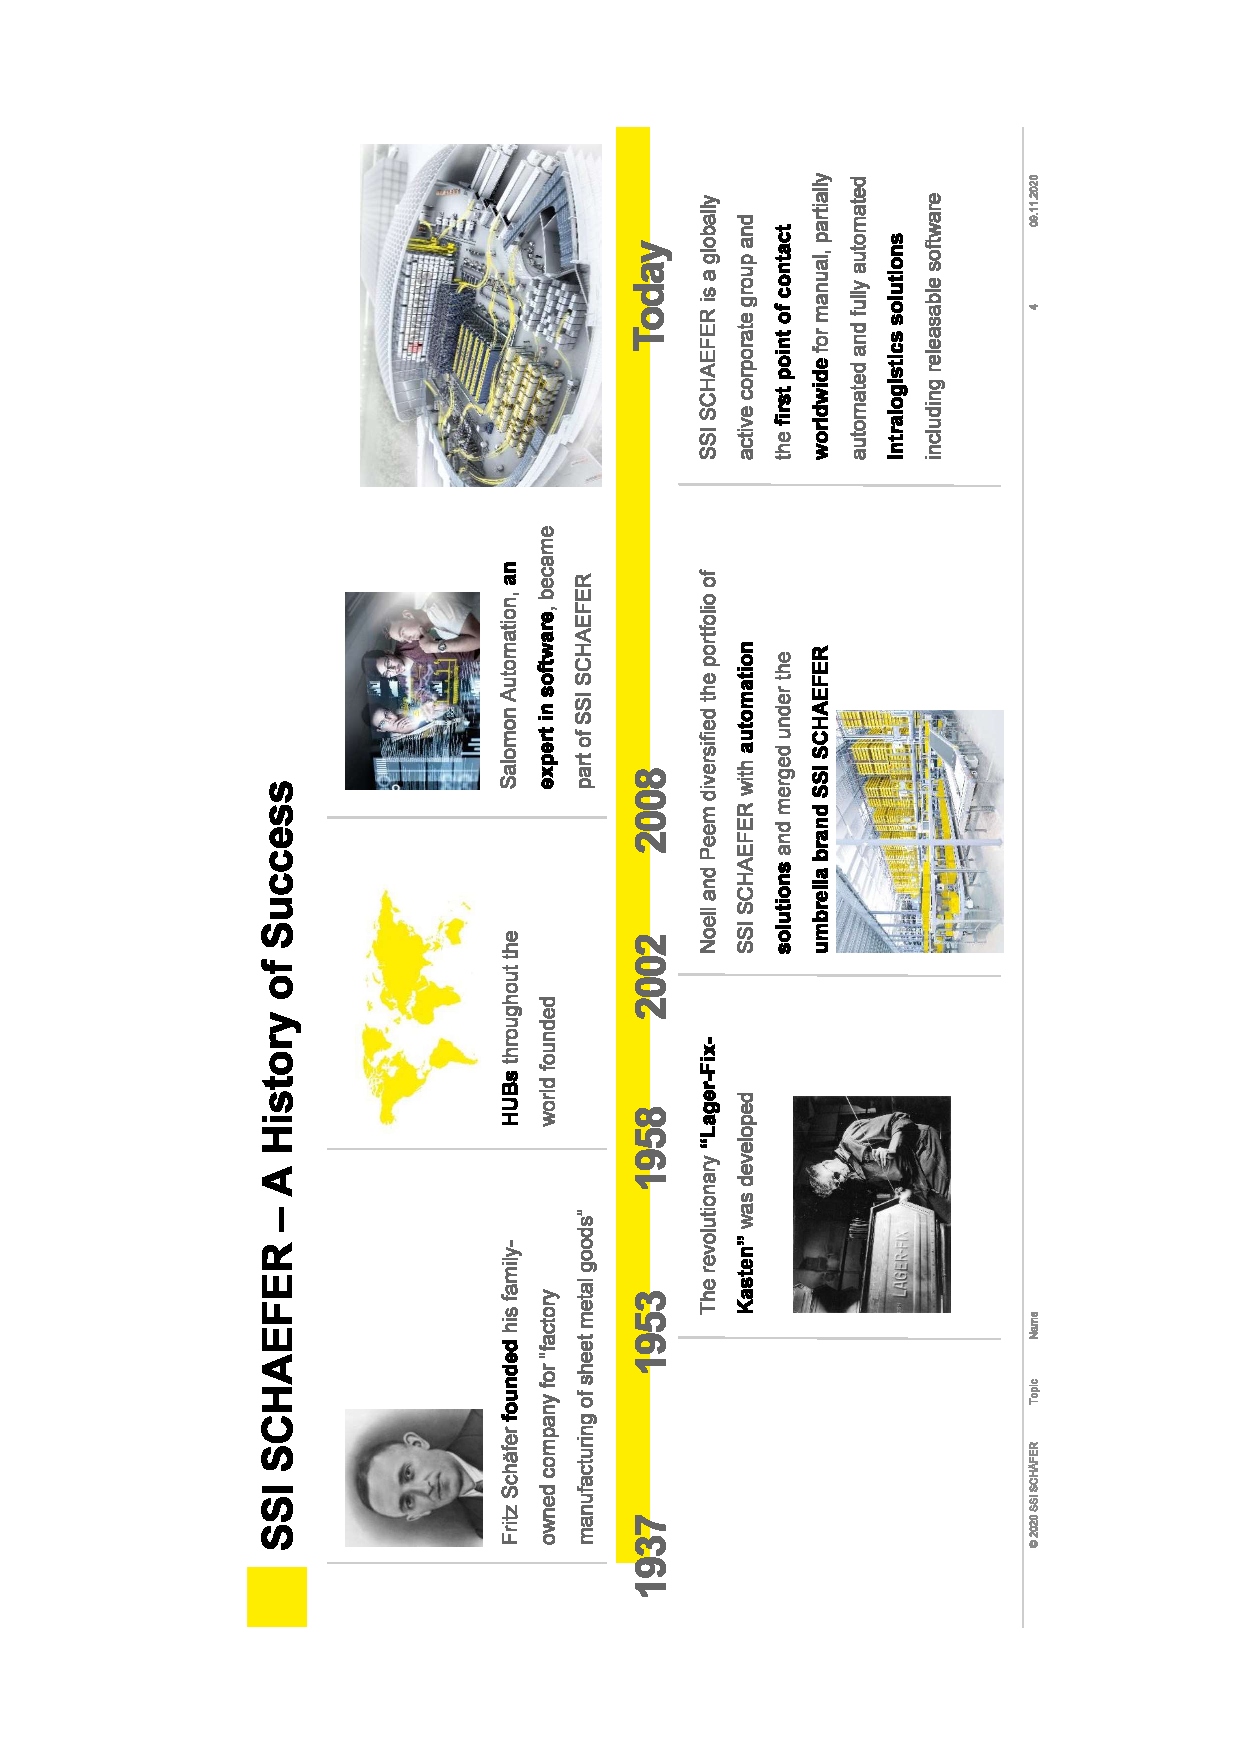
\includegraphics[width=0.8\linewidth]{images/history.pdf}

		\newpage
		\subsection{Carte des filiales SSI SCHÄFER}\label{appendix:map}
			%\includegraphics[width=0.8\textwidth]{tikzpgf.pdf}
			\begin{center}
				\includegraphics[width=\textwidth]{images/world_map.jpg}
			\end{center}
				%\includegraphics[width=\textwidth]{world_map.jpg}
		\newpage


		\subsection{Liste complète des fonctionnalités de MORPHEUS WMS}\label{appendix:morpheusWMSFonctionnalites}
		%\addcontentsline{toc}{subsection}{Annexe 1}
			%pour les screens issus du site internet à voir avec Charlotte si elle a les images 
			% + voir si juste mettre source interne ..
			% lui demander schéma WMS / WCS
			% + histoire schaefer...
			\begin{figure}[h!]
					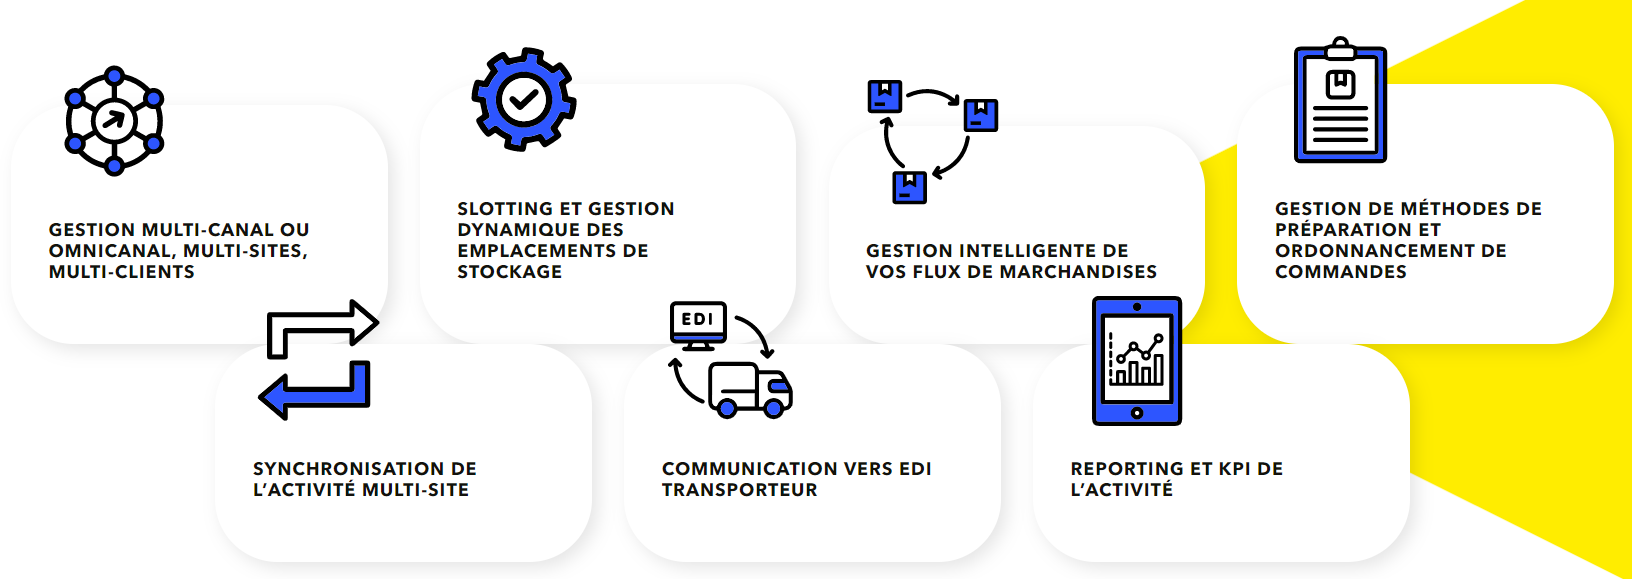
\includegraphics[width=\linewidth]{images/morpheus_wms_fonctionnalites.png}
					\caption{Fonctionnalités de Morpheus WMS}%\cite{screenshot}
					\label{fig:morpheus_wms_fonctionnalites}
			\end{figure}
		\subsection{Liste complète des fonctionnalités de MORPHEUS WCS}\label{appendix:morpheusWCSFonctionnalites}
		%\addcontentsline{toc}{subsection}{Annexe 2}
			\begin{figure}[h!]
					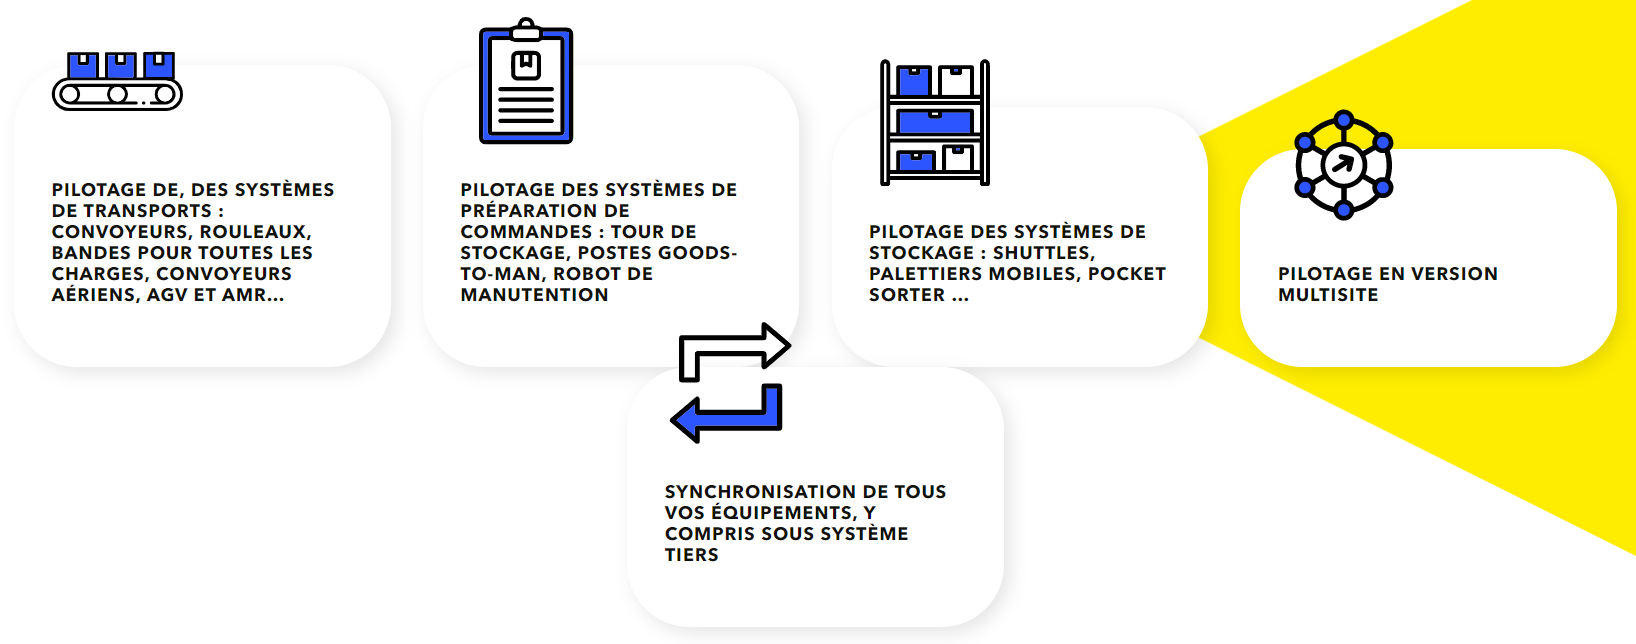
\includegraphics[width=\linewidth]{images/morpheus_wcs_fonctionnalites.png}
					\caption{Fonctionnalités de Morpheus WCS}%\cite{screenshot}
					\label{fig:morpheus_wcs_fonctionnalites}
			\end{figure}

		\newpage

		\subsection{Écrans de l'application}\label{appendix:application}
			\begin{figure}[h!]
				\begin{center}
					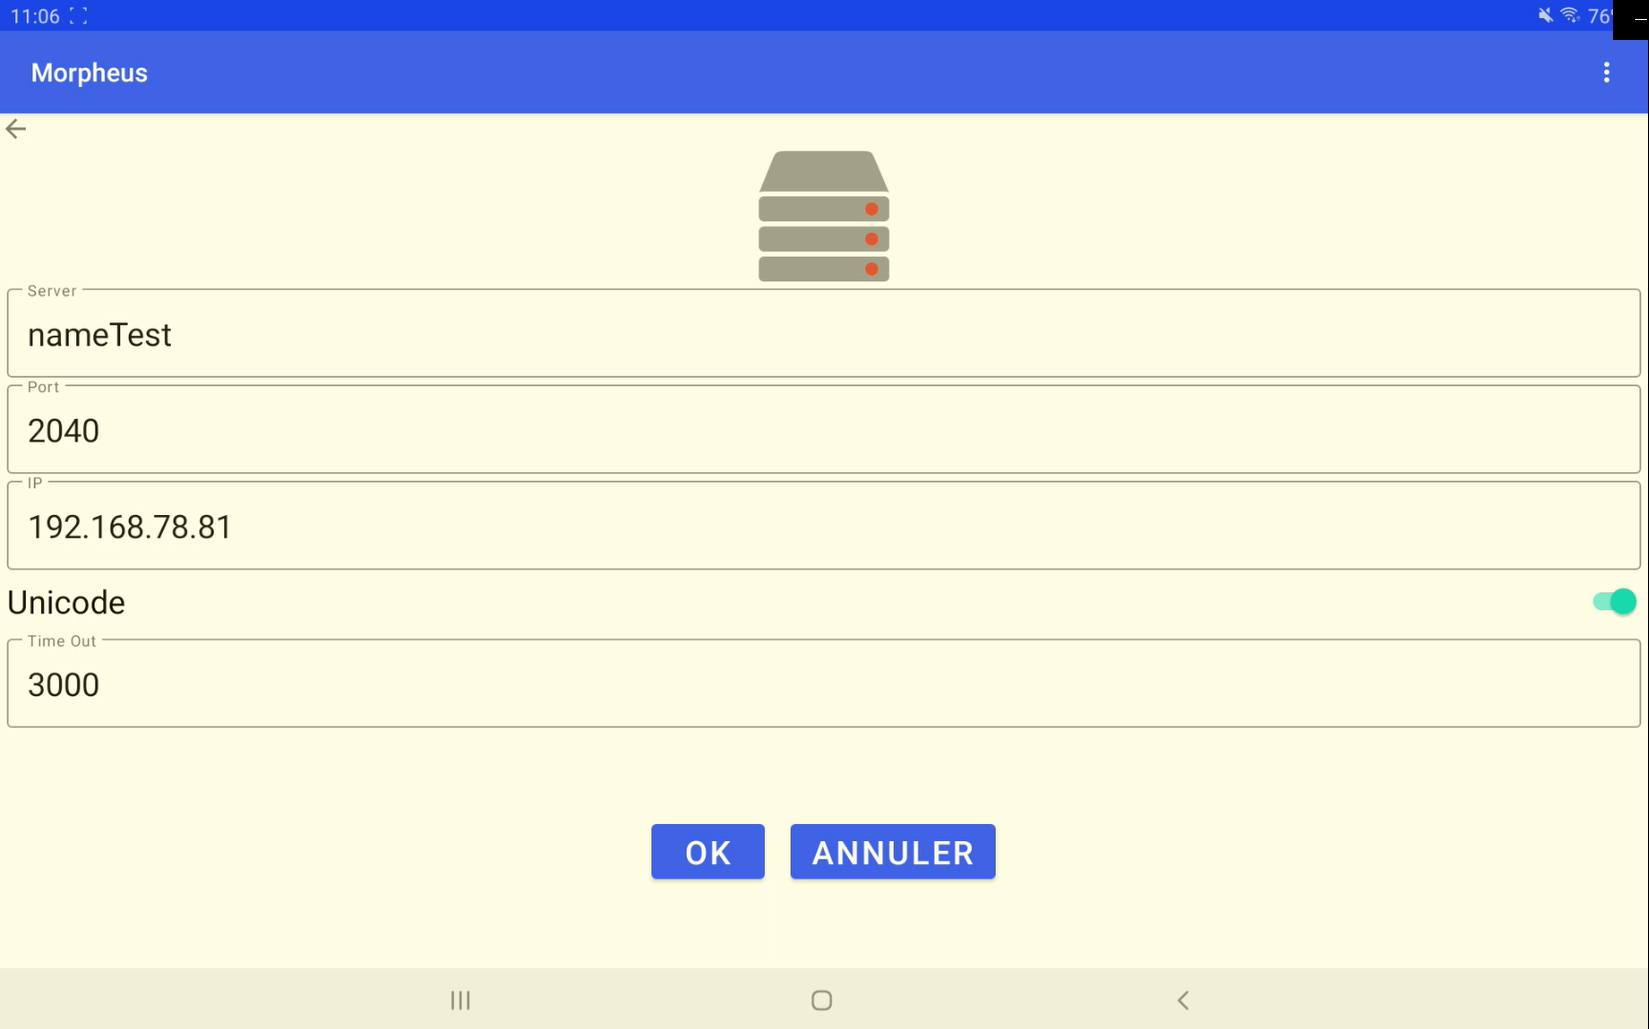
\includegraphics[width=0.7\linewidth]{application/config_socket.PNG}
				\end{center}
				\caption{Écran de configuration du socket}
				\label{fig:applications:config_socket}
			\end{figure}	

			\vfill

			\begin{figure}[h!]
				\begin{center}
					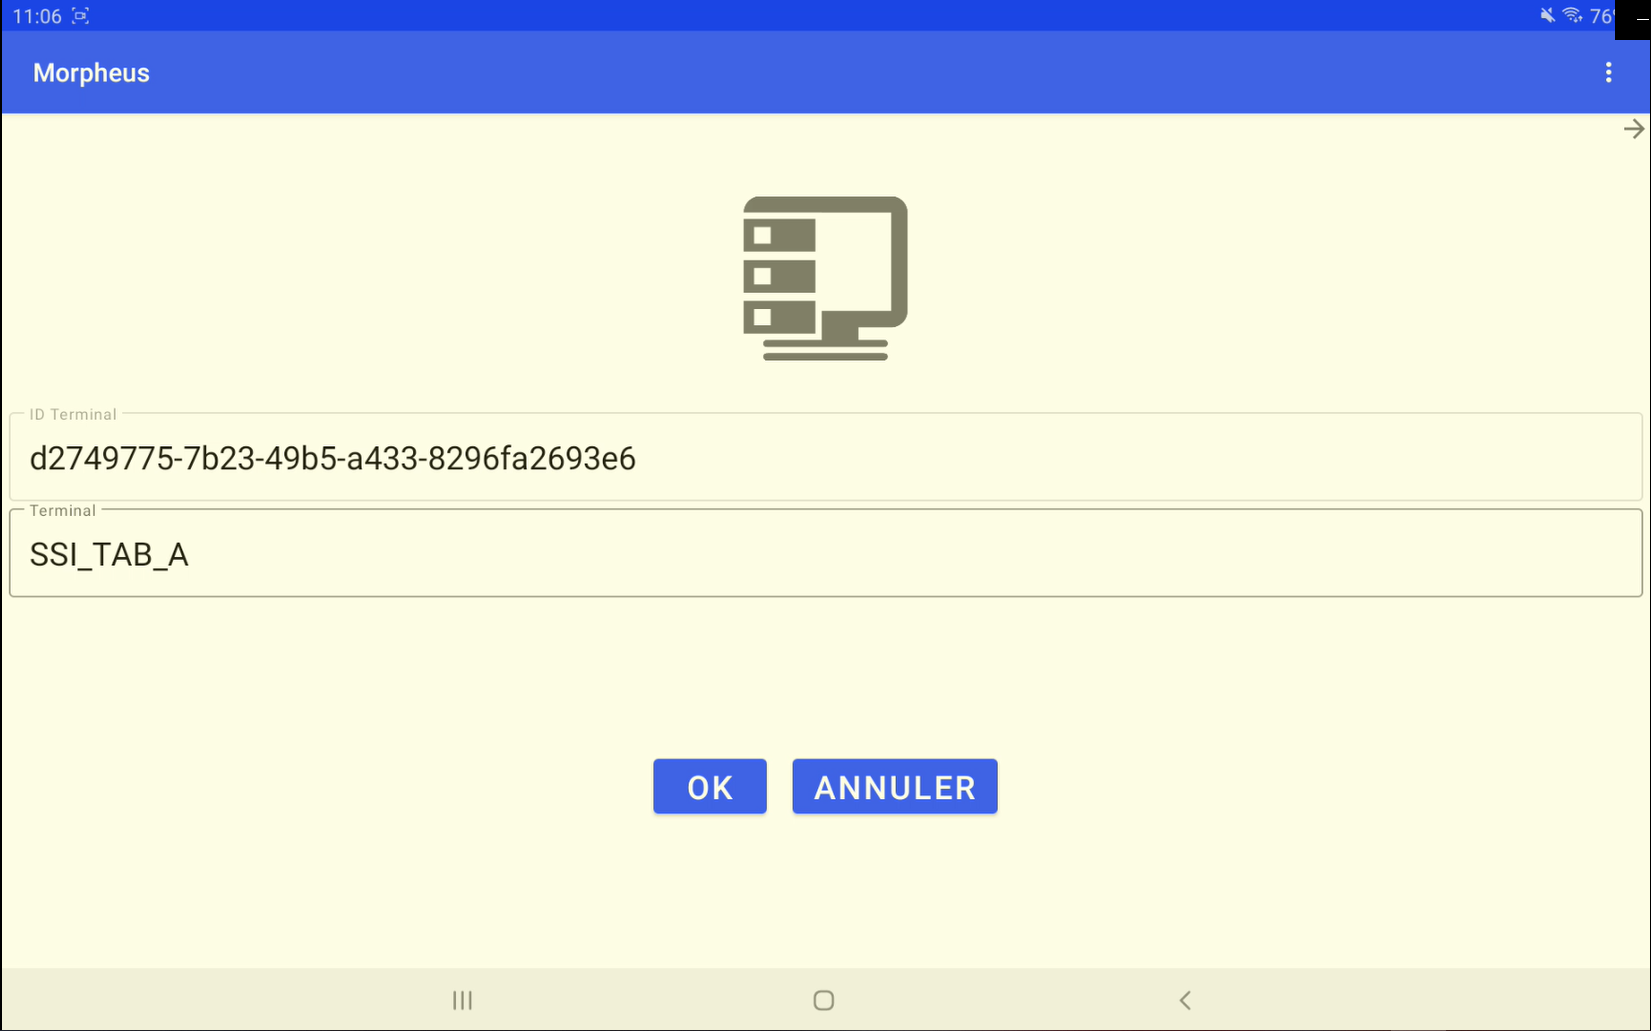
\includegraphics[width=0.7\linewidth]{application/config_terminal.PNG}
				\end{center}
				\caption{Écran de configuration du terminal}
				\label{fig:applications:config_terminal}
			\end{figure}	

		\newpage

			\begin{figure}[h!]
				\begin{center}
					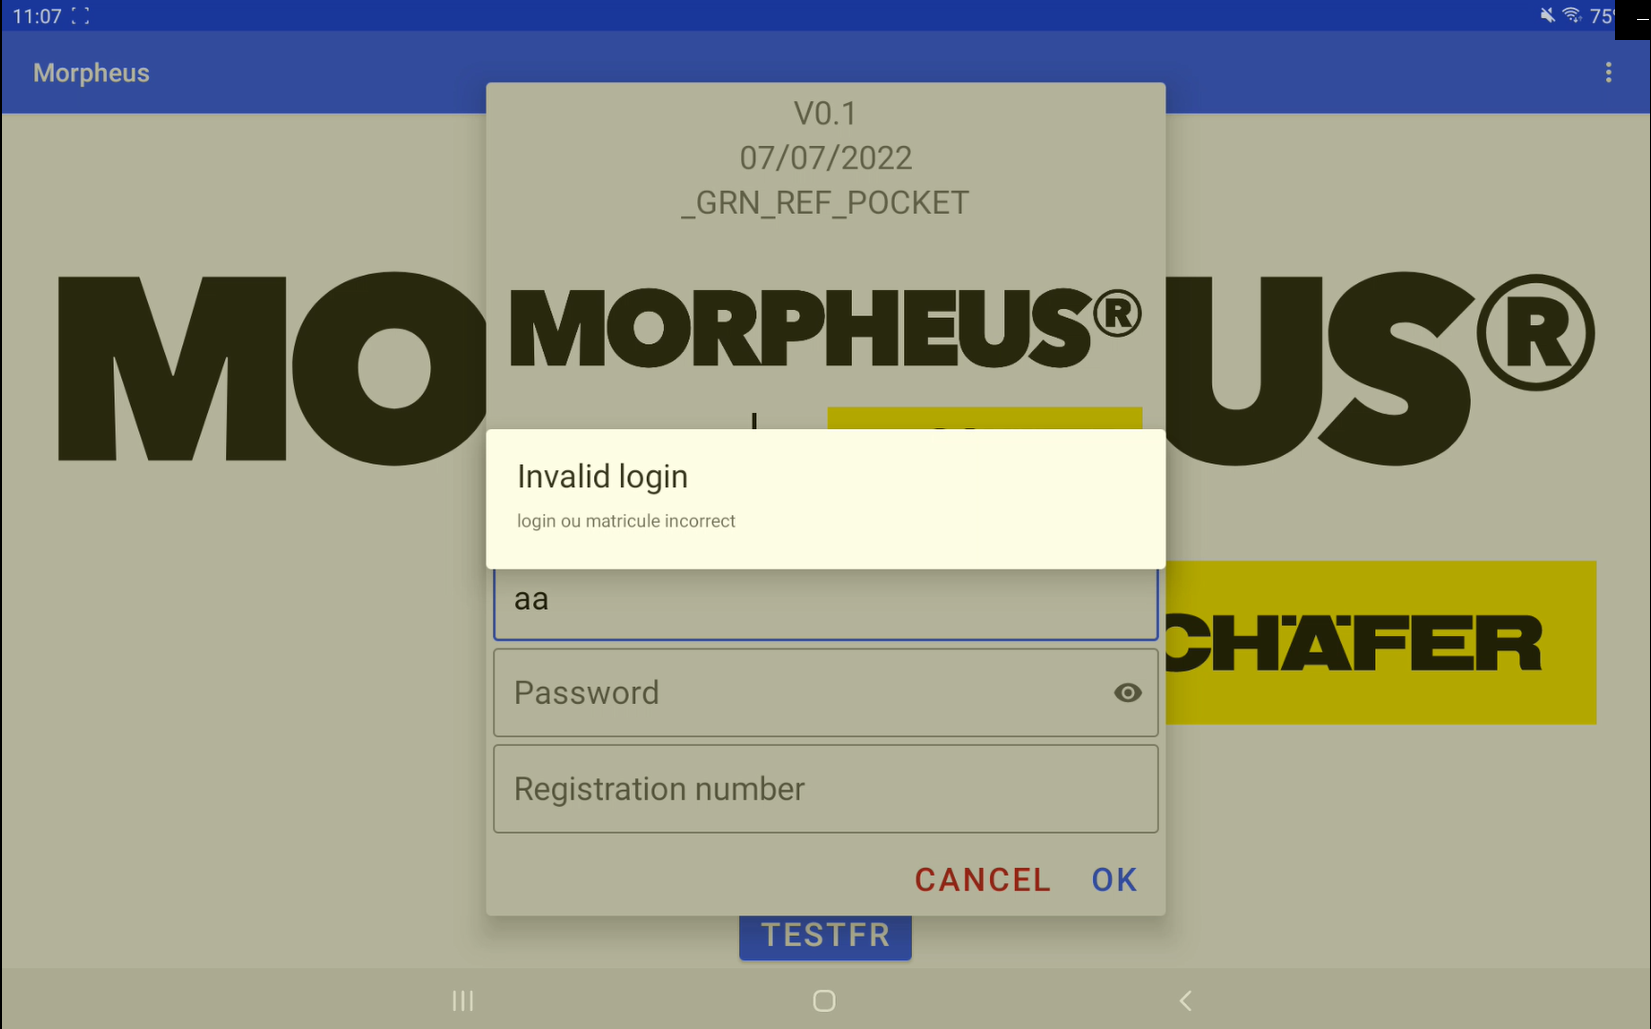
\includegraphics[width=0.7\linewidth]{application/error_message.PNG}
				\end{center}
				\caption{Écran de message d'erreur}
				\label{fig:applications:error_message}
			\end{figure}	

			\vfill

			\begin{figure}[h!]
				\begin{center}
					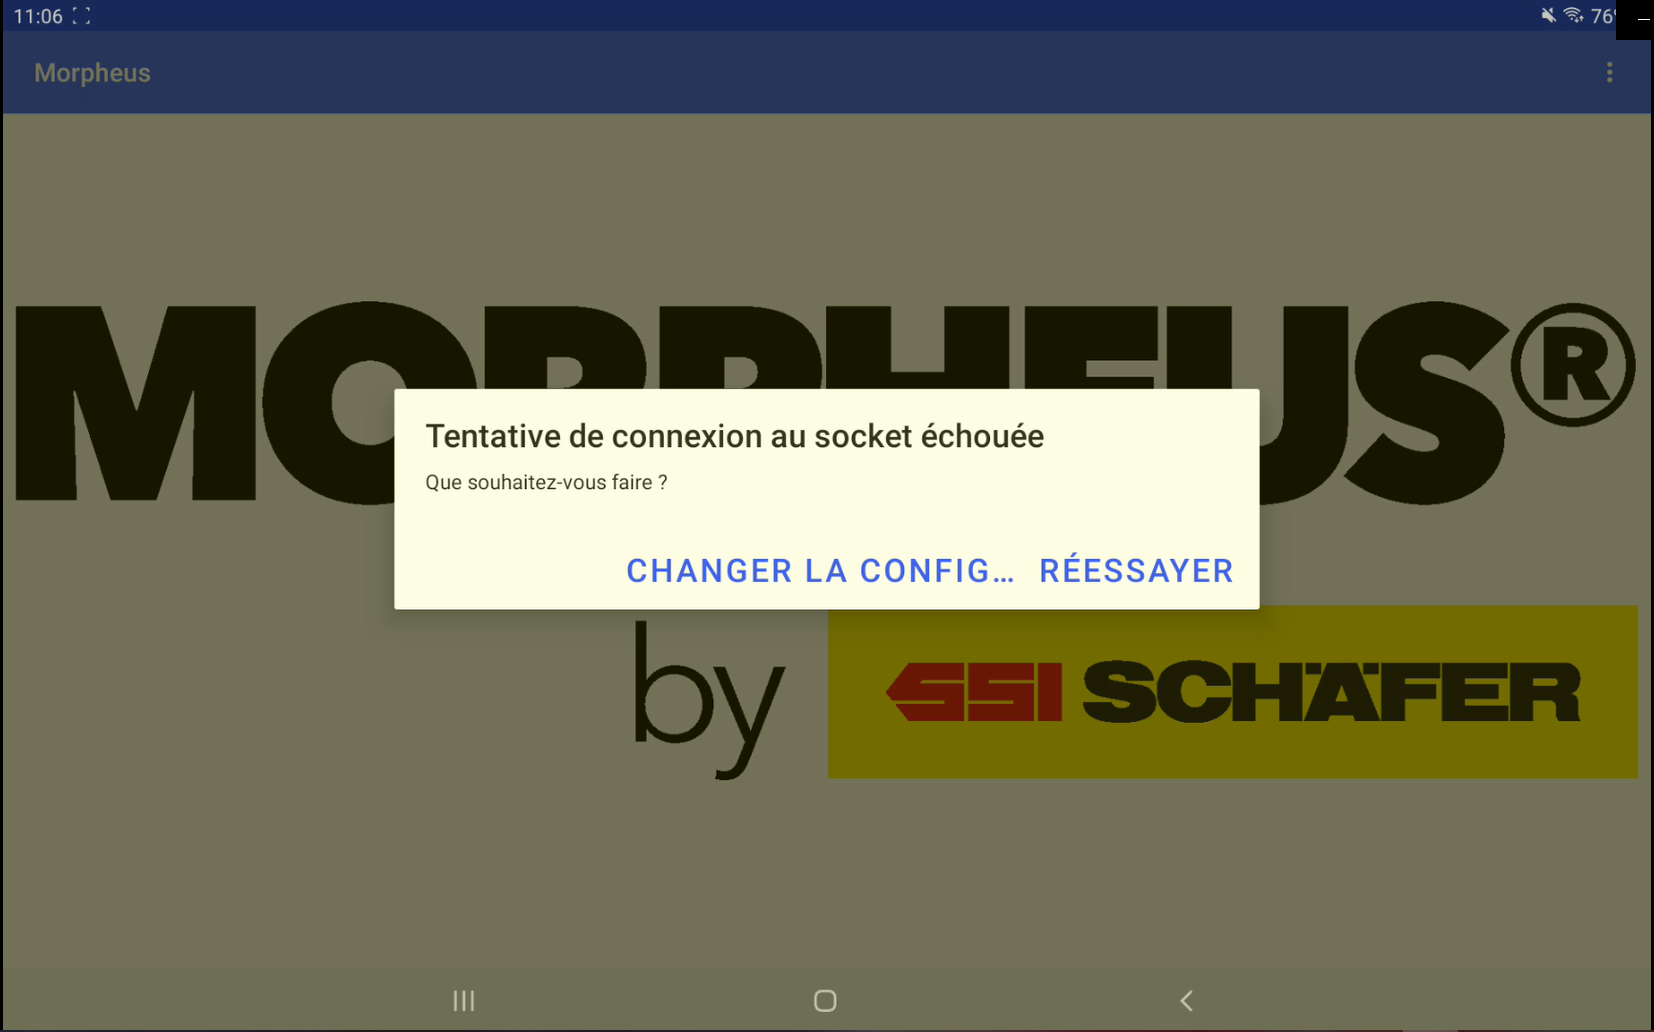
\includegraphics[width=0.7\linewidth]{application/fail.PNG}
				\end{center}
				\caption{Écran lors de l'échec de la connexion au socket}
				\label{fig:applications:fail}
			\end{figure}	

		\newpage

			\begin{figure}[h!]
				\begin{center}
					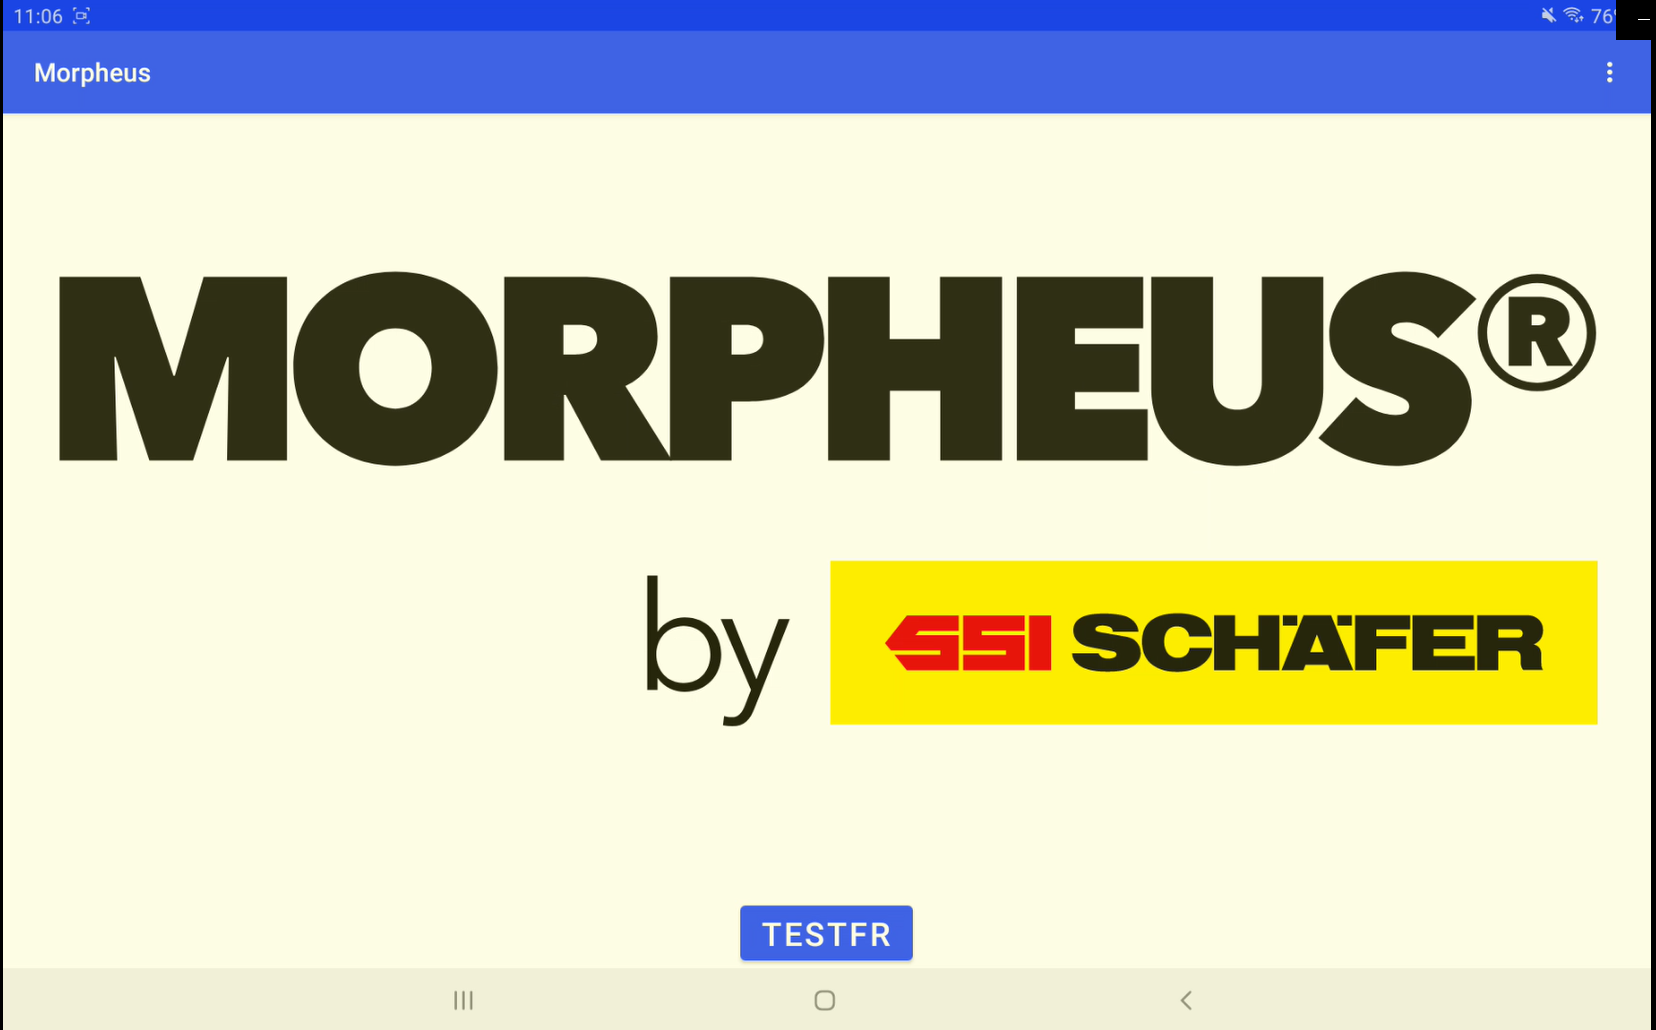
\includegraphics[width=0.7\linewidth]{application/home.PNG}
				\end{center}
				\caption{Écran d'accueil}
				\label{fig:applications:home}
			\end{figure}	

			\vfill

			\begin{figure}[h!]
				\begin{center}
					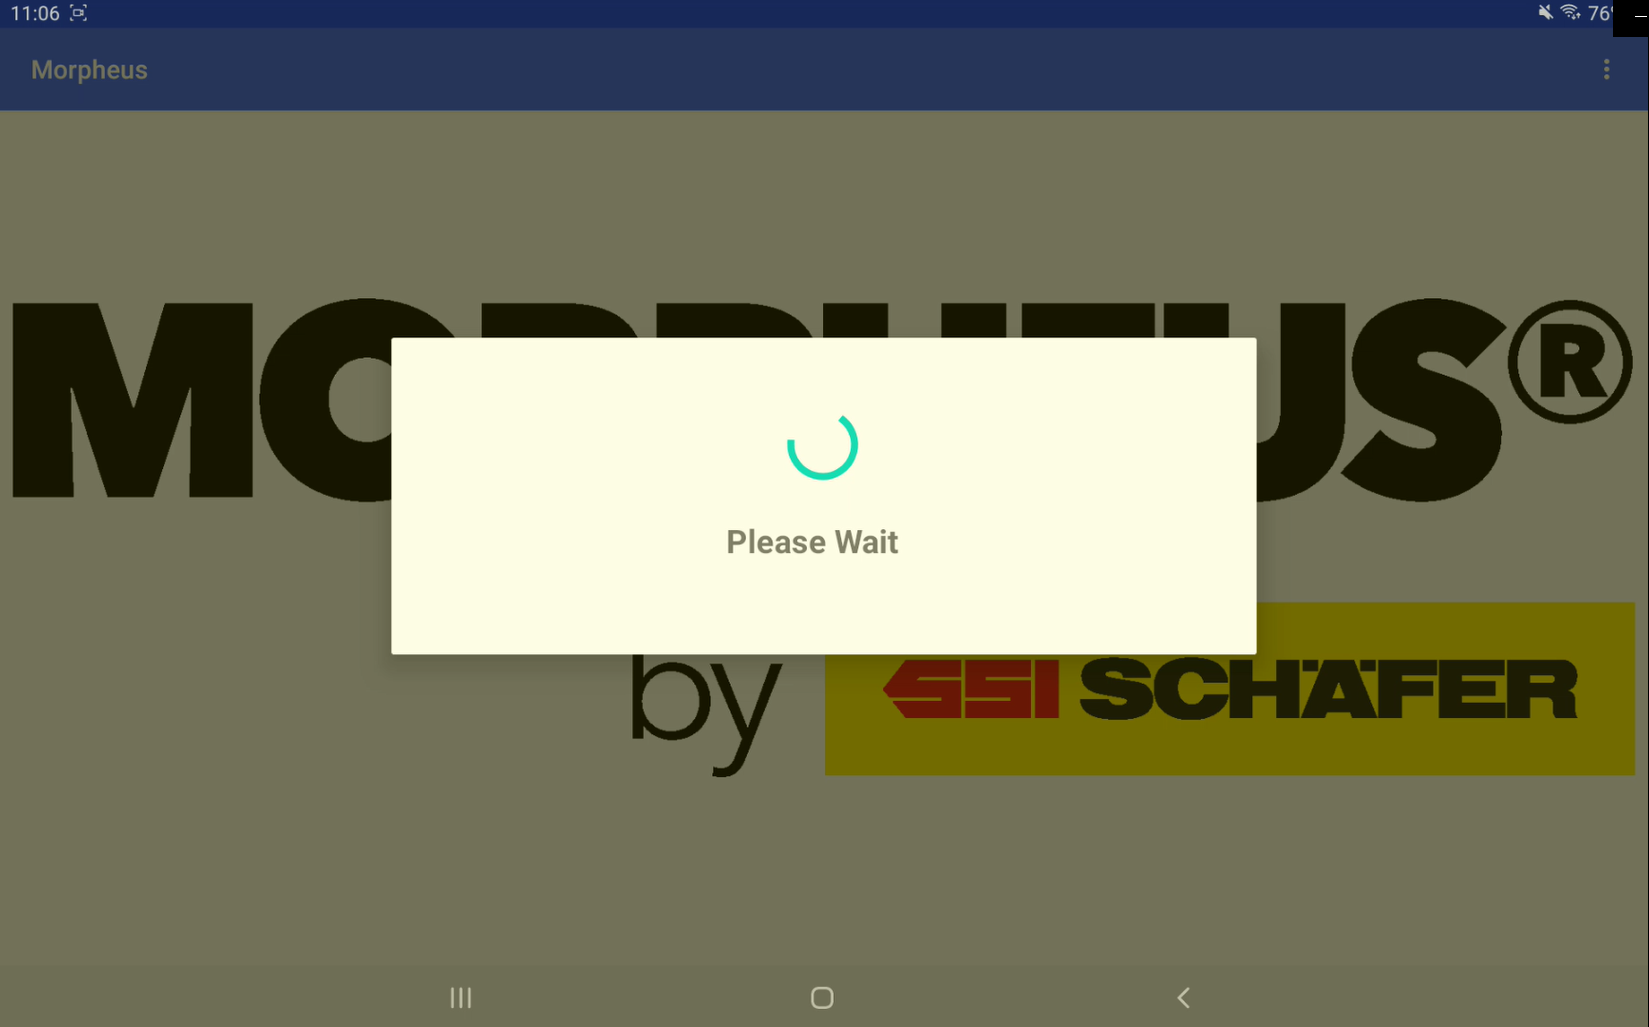
\includegraphics[width=0.7\linewidth]{application/loading.PNG}
				\end{center}
				\caption{Écran de chargement}
				\label{fig:applications:loading}
			\end{figure}	

		\newpage

			\begin{figure}[h!]
				\begin{center}
					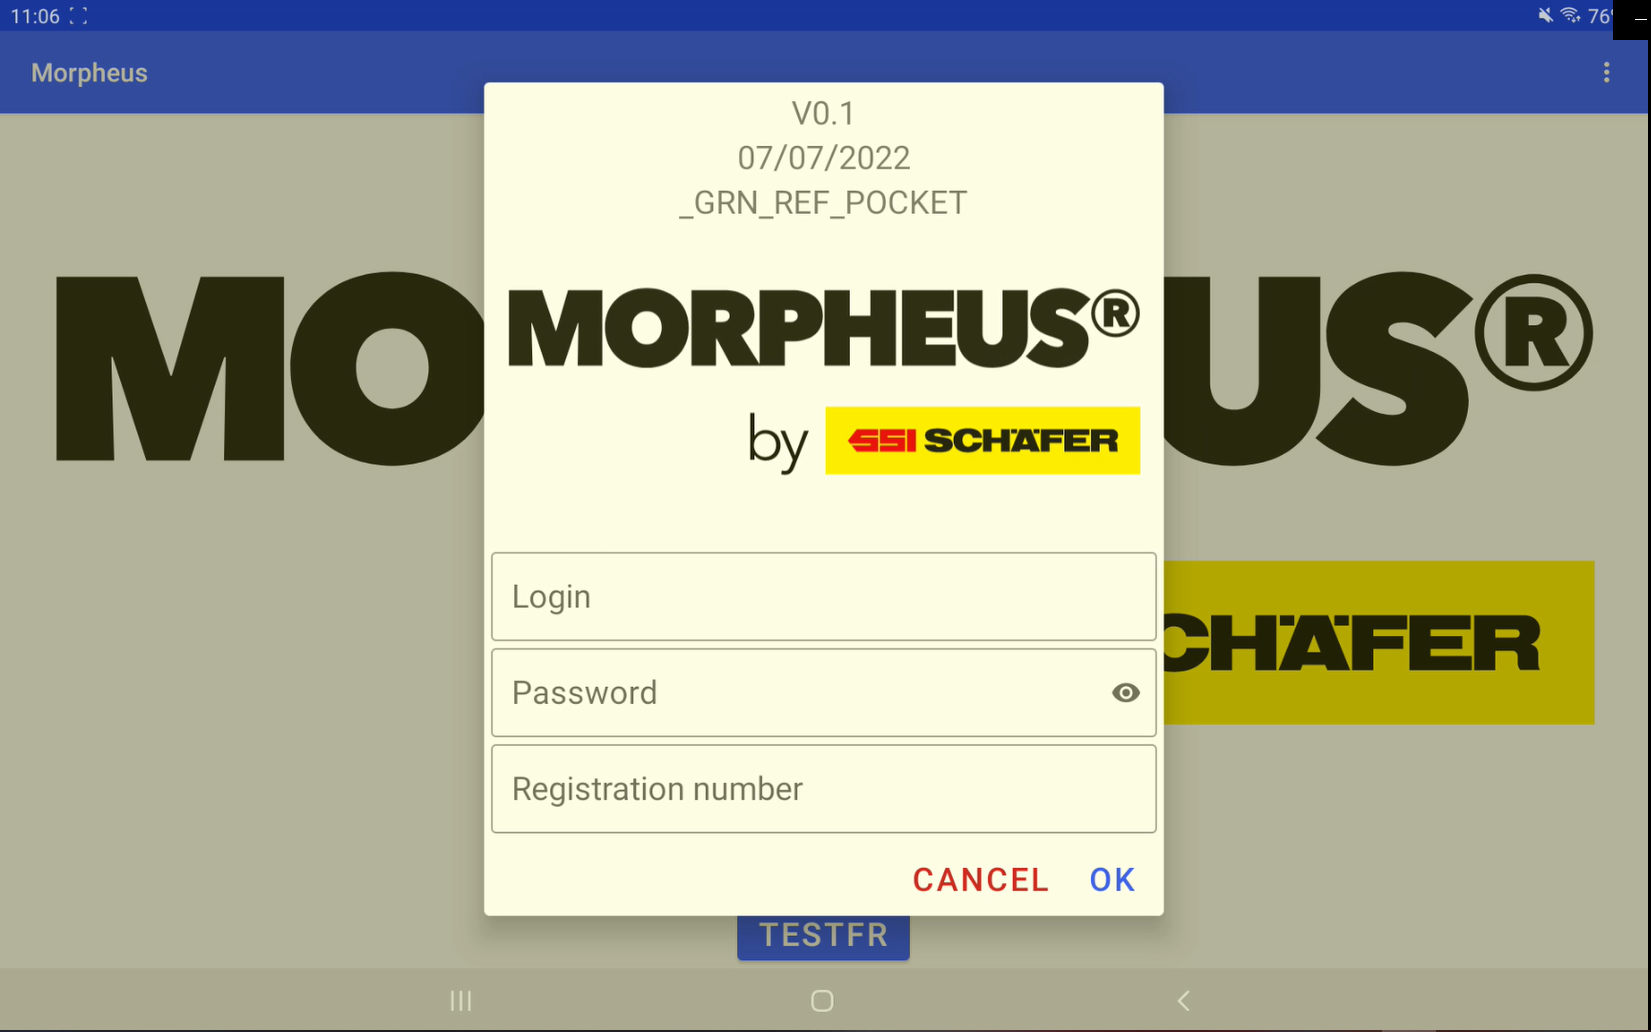
\includegraphics[width=0.7\linewidth]{application/login.PNG}
				\end{center}
				\caption{Écran de connexion}
				\label{fig:applications:login}
			\end{figure}	

			\vfill

			\begin{figure}[h!]
				\begin{center}
					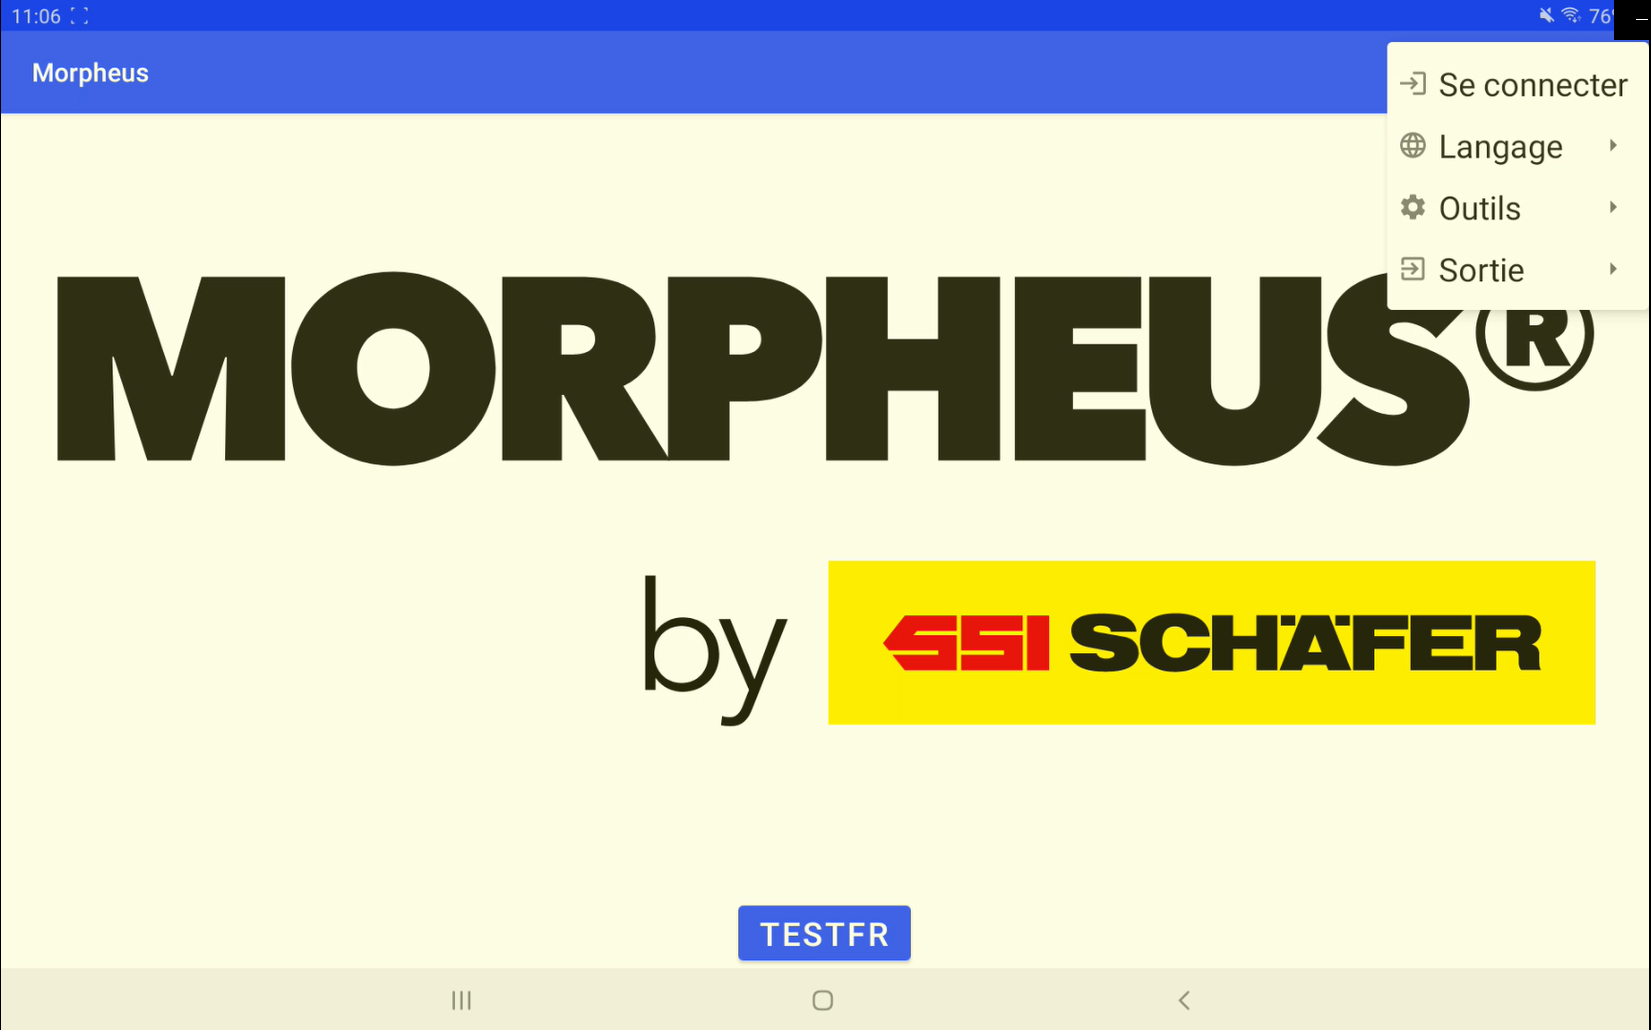
\includegraphics[width=0.7\linewidth]{application/menu.PNG}
				\end{center}
				\caption{Écran du menu}
				\label{fig:applications:menu}
			\end{figure}	

		\newpage

			\begin{figure}[h!]
				\begin{center}
					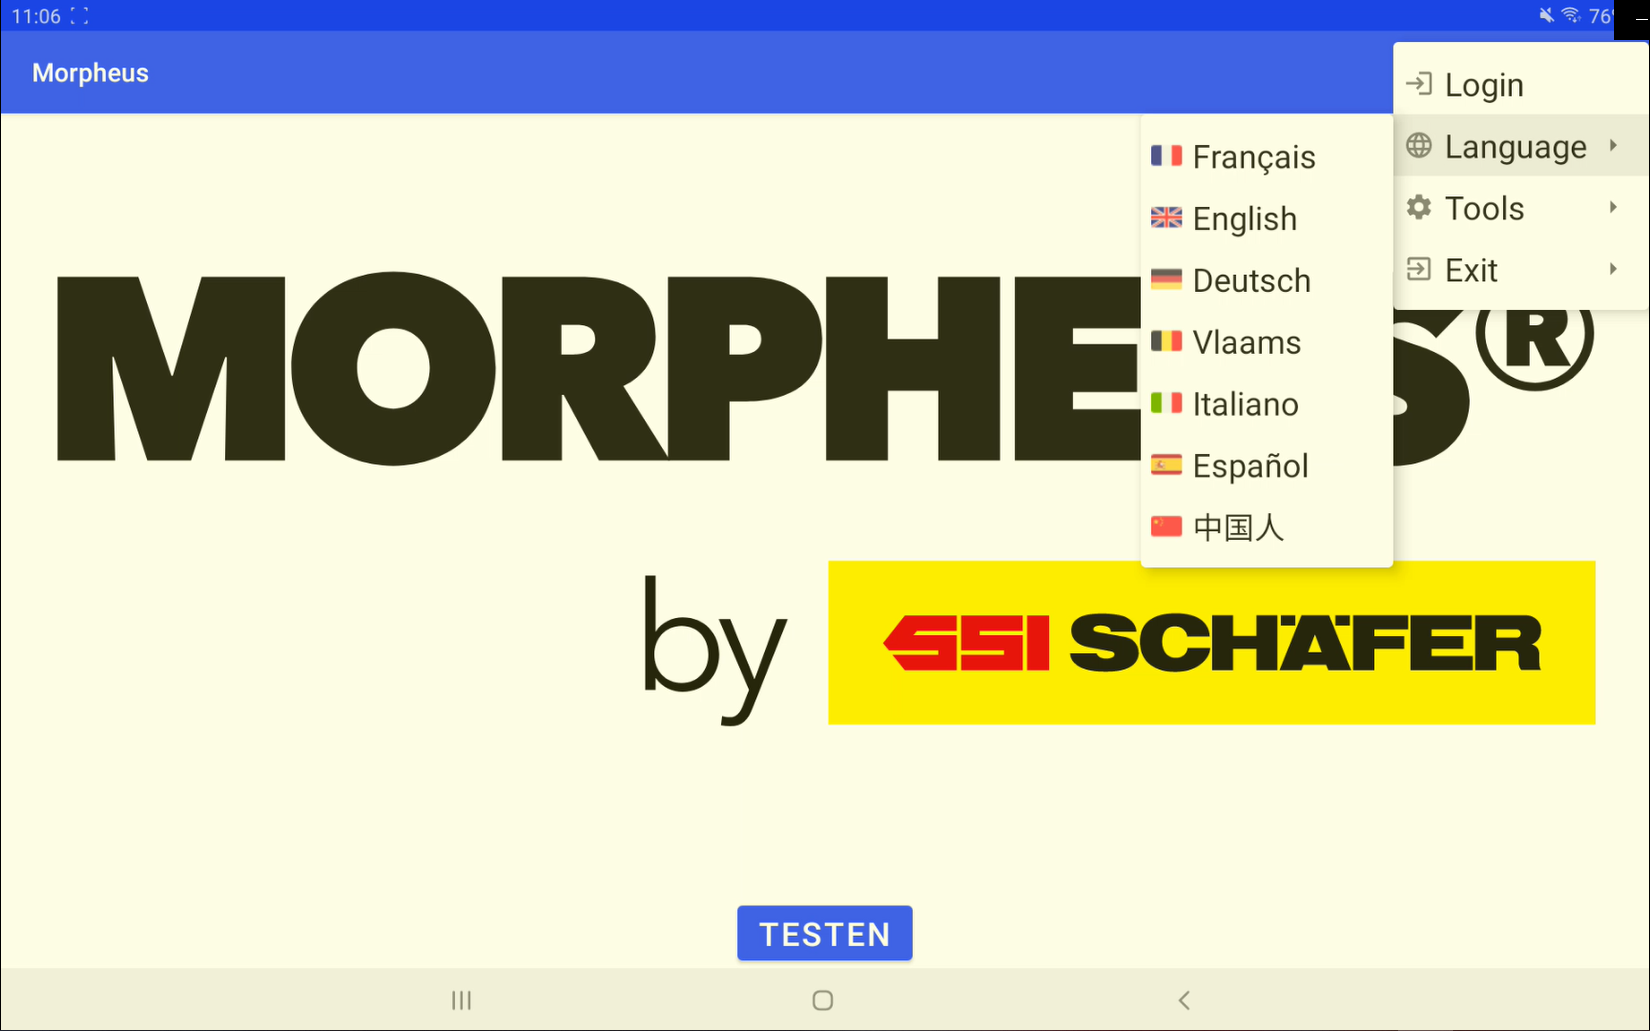
\includegraphics[width=0.7\linewidth]{application/menu_en_language.PNG}
				\end{center}
				\caption{Écran du menu langage en anglais}
				\label{fig:applications:menu_en_language}
			\end{figure}	

			\vfill

			\begin{figure}[h!]
				\begin{center}
					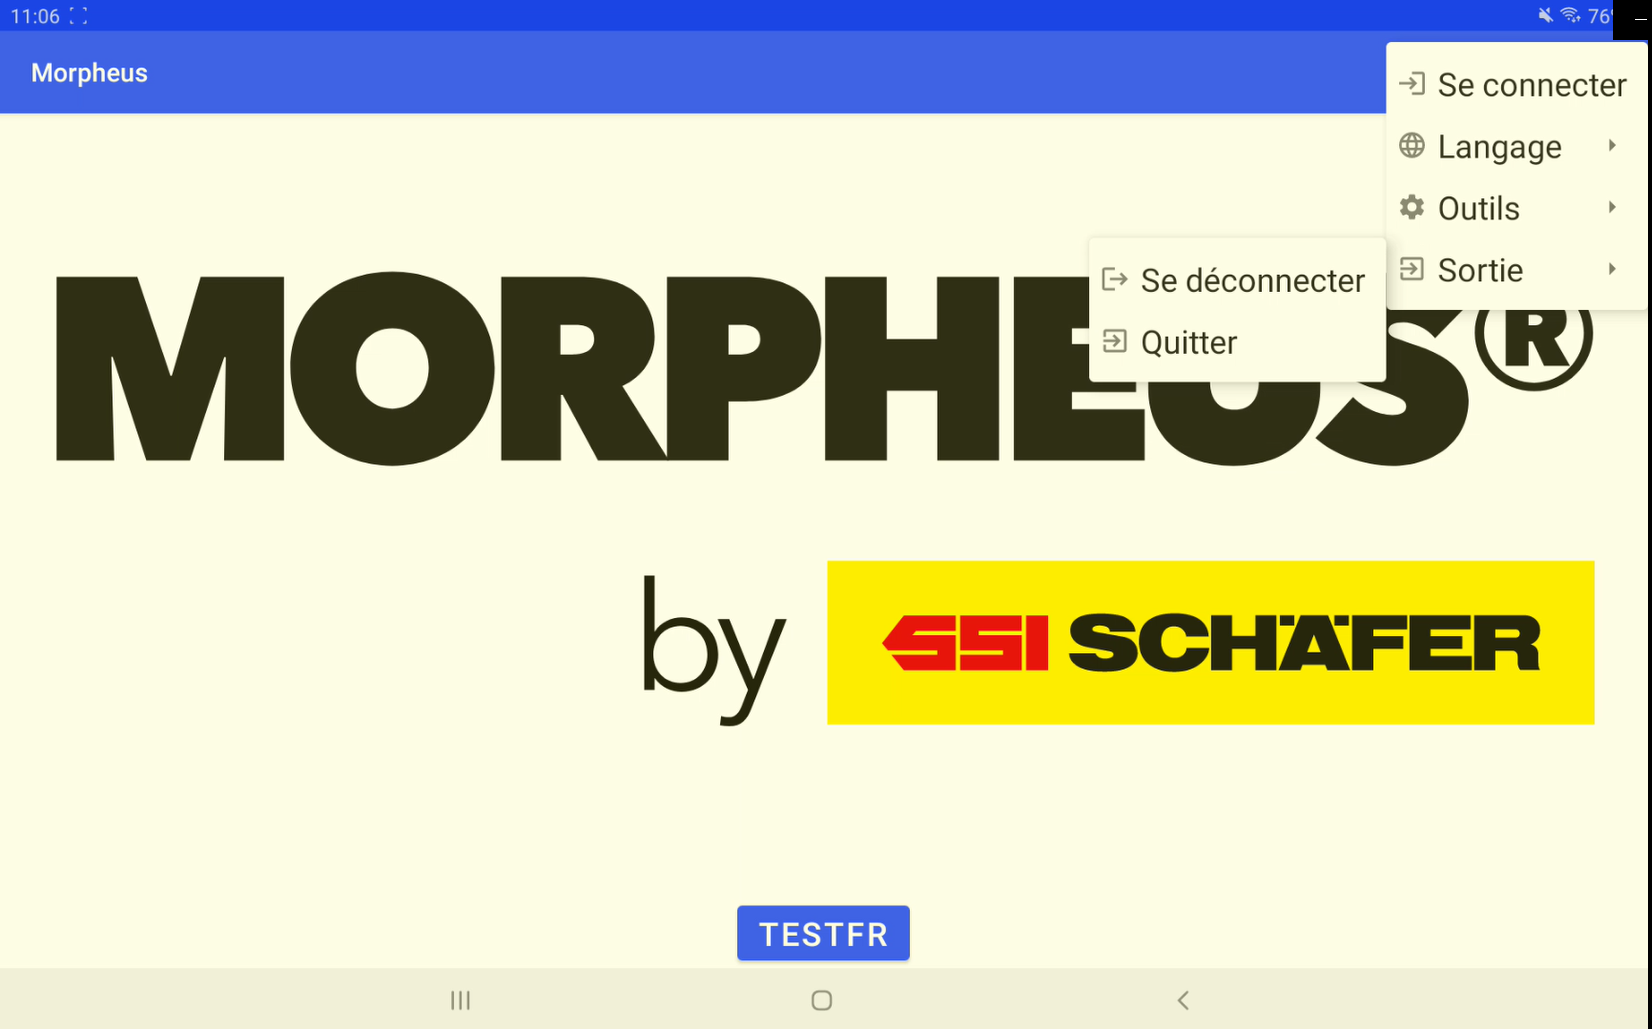
\includegraphics[width=0.7\linewidth]{application/menu_exit.PNG}
				\end{center}
				\caption{Écran du menu sortie}
				\label{fig:applications:menu_exit}
			\end{figure}	

		\newpage

			\begin{figure}[h!]
				\begin{center}
					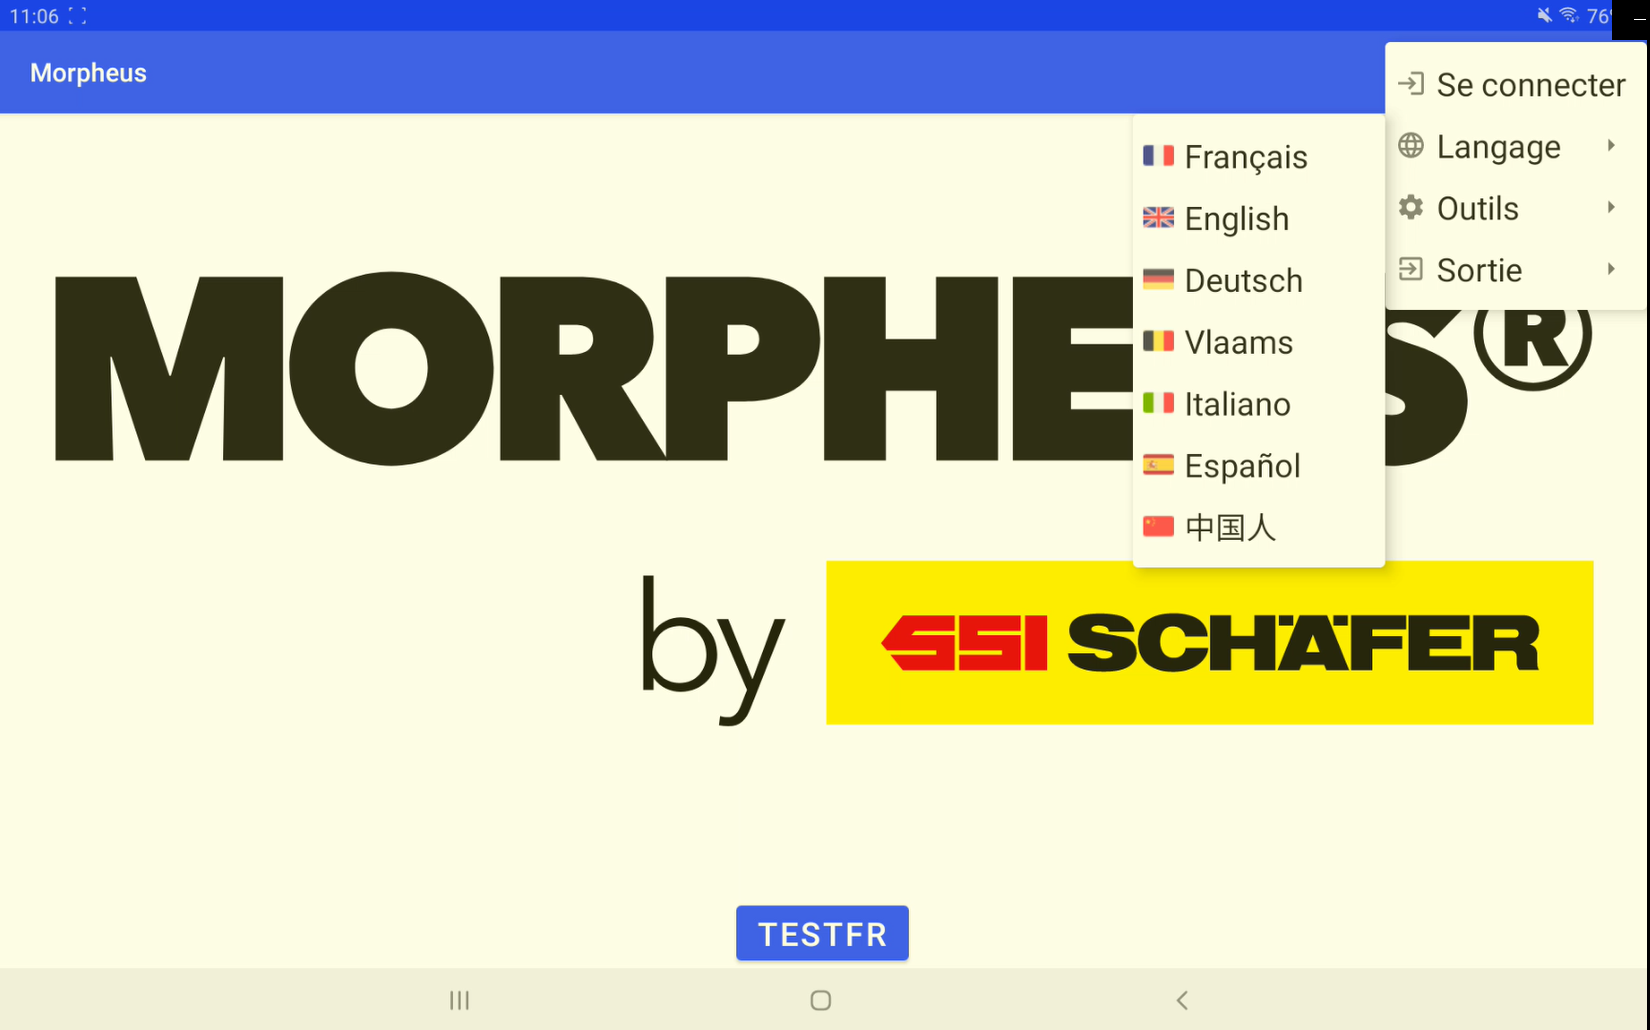
\includegraphics[width=0.7\linewidth]{application/menu_language.PNG}
				\end{center}
				\caption{Écran du menu langage}
				\label{fig:applications:menu_language}
			\end{figure}	

			\vfill

			\begin{figure}[h!]
				\begin{center}
					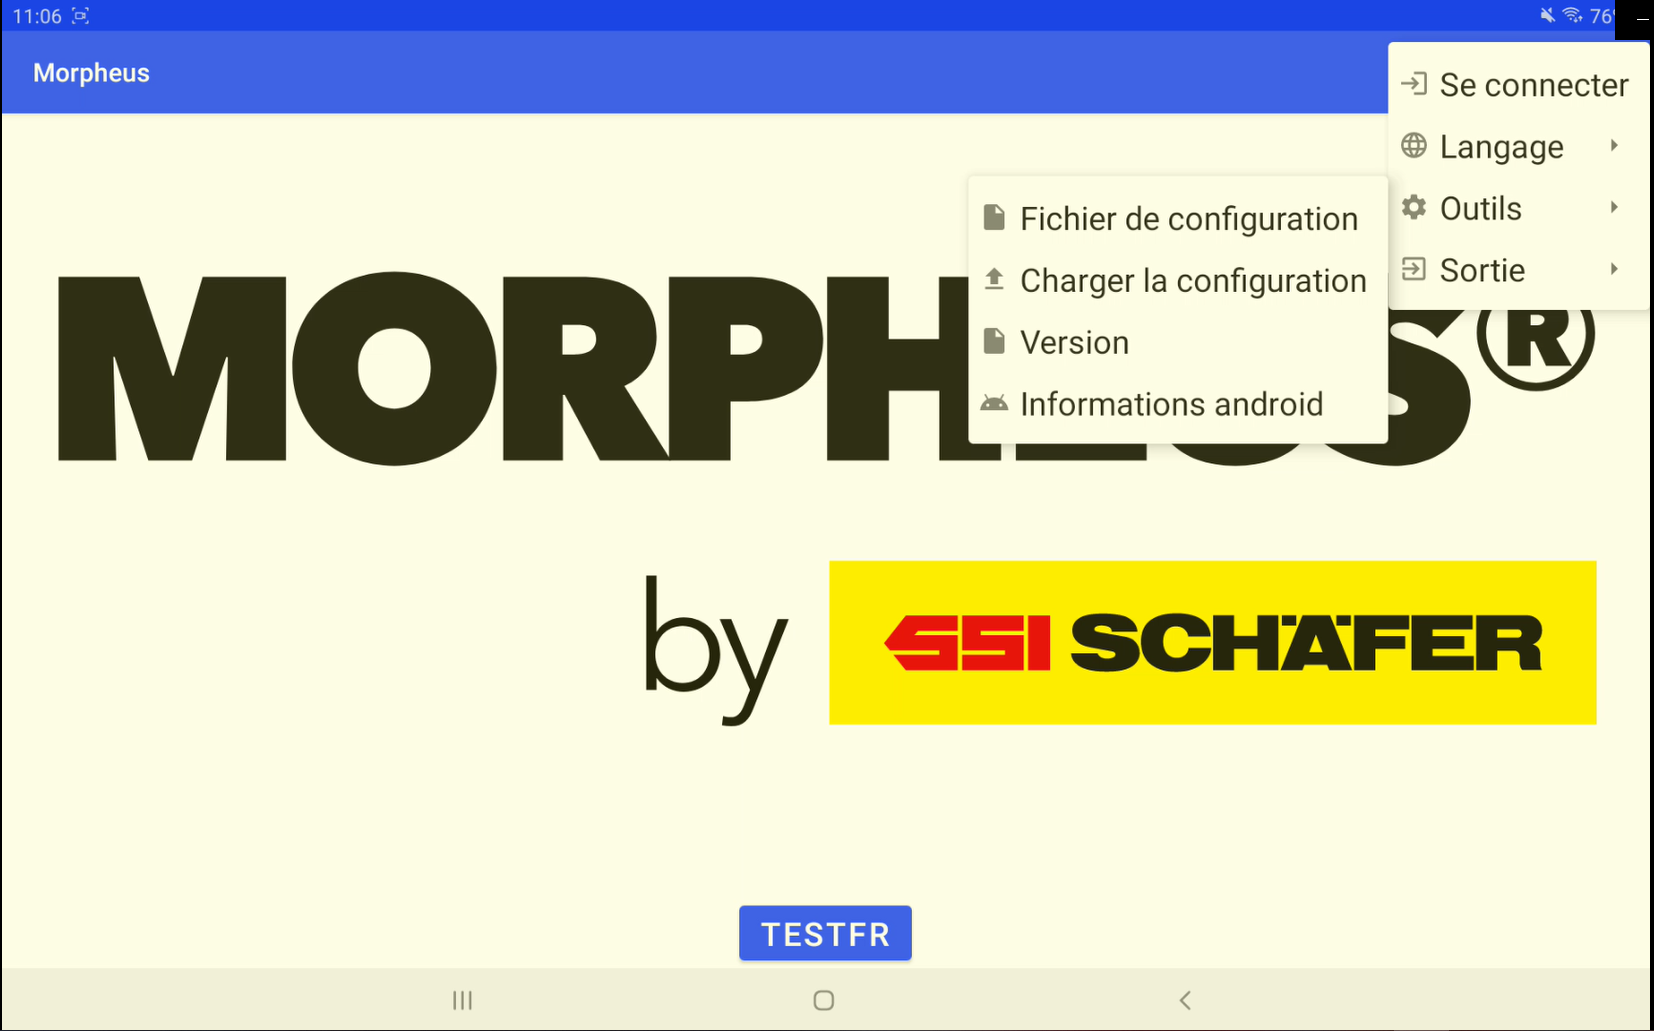
\includegraphics[width=0.7\linewidth]{application/menu_tools.PNG}
				\end{center}
				\caption{Écran du menu outils}
				\label{fig:applications:menu_tools}
			\end{figure}	

		\newpage

			\begin{figure}[h!]
				\begin{center}
					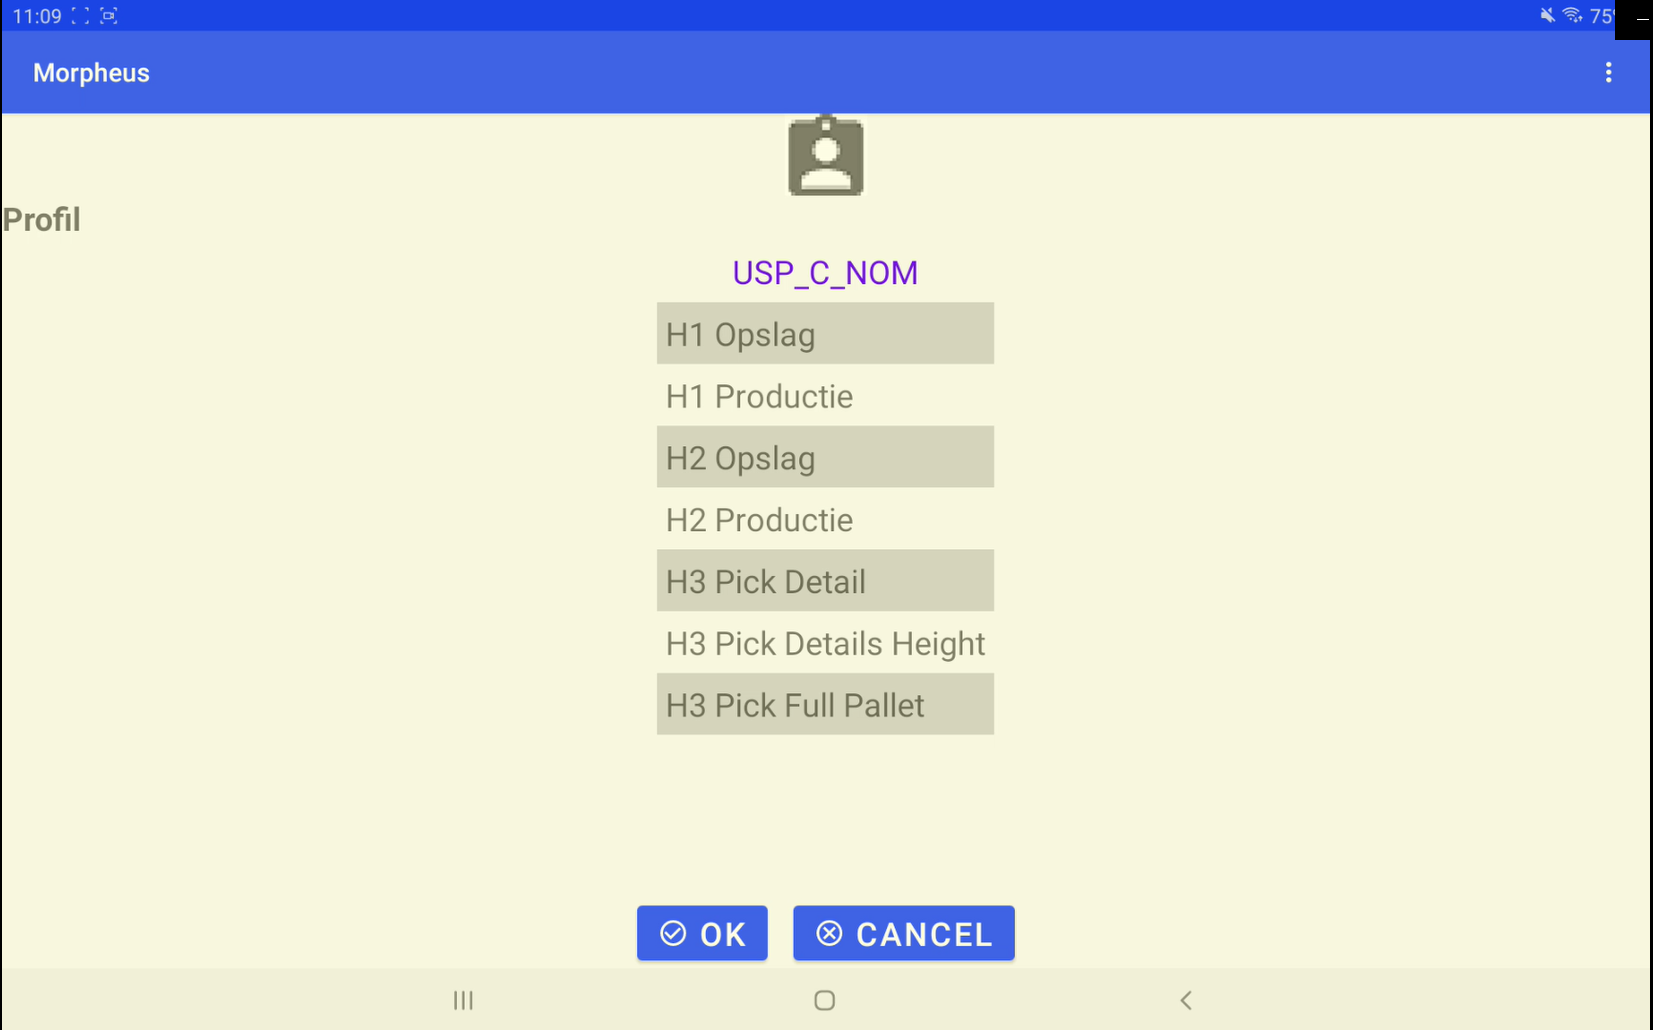
\includegraphics[width=0.7\linewidth]{application/profile.PNG}
				\end{center}
				\caption{Écran de sélection du profil}
				\label{fig:applications:profile}
			\end{figure}	

			\vfill

			\begin{figure}[h!]
				\begin{center}
					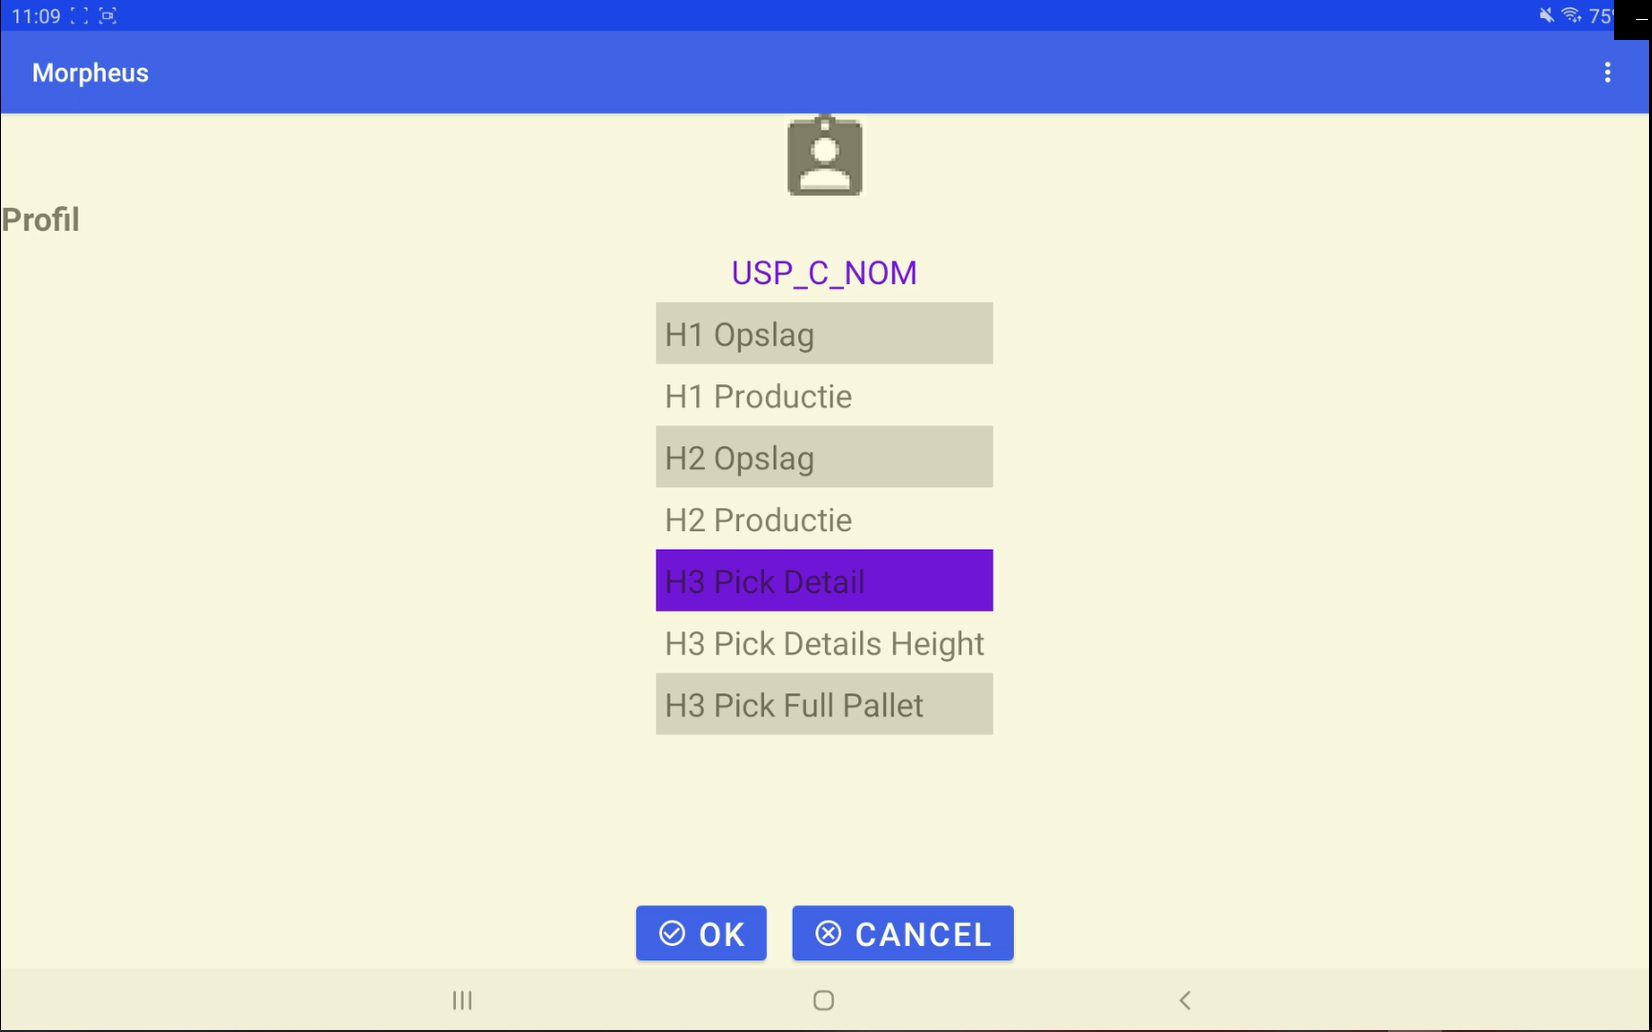
\includegraphics[width=0.7\linewidth]{application/profile_selected.PNG}
				\end{center}
				\caption{Écran de sélection du profil : un profil est sélectionné}
				\label{fig:applications:profile_selected}
			\end{figure}	

		\newpage

			\begin{figure}[h!]
				\begin{center}
					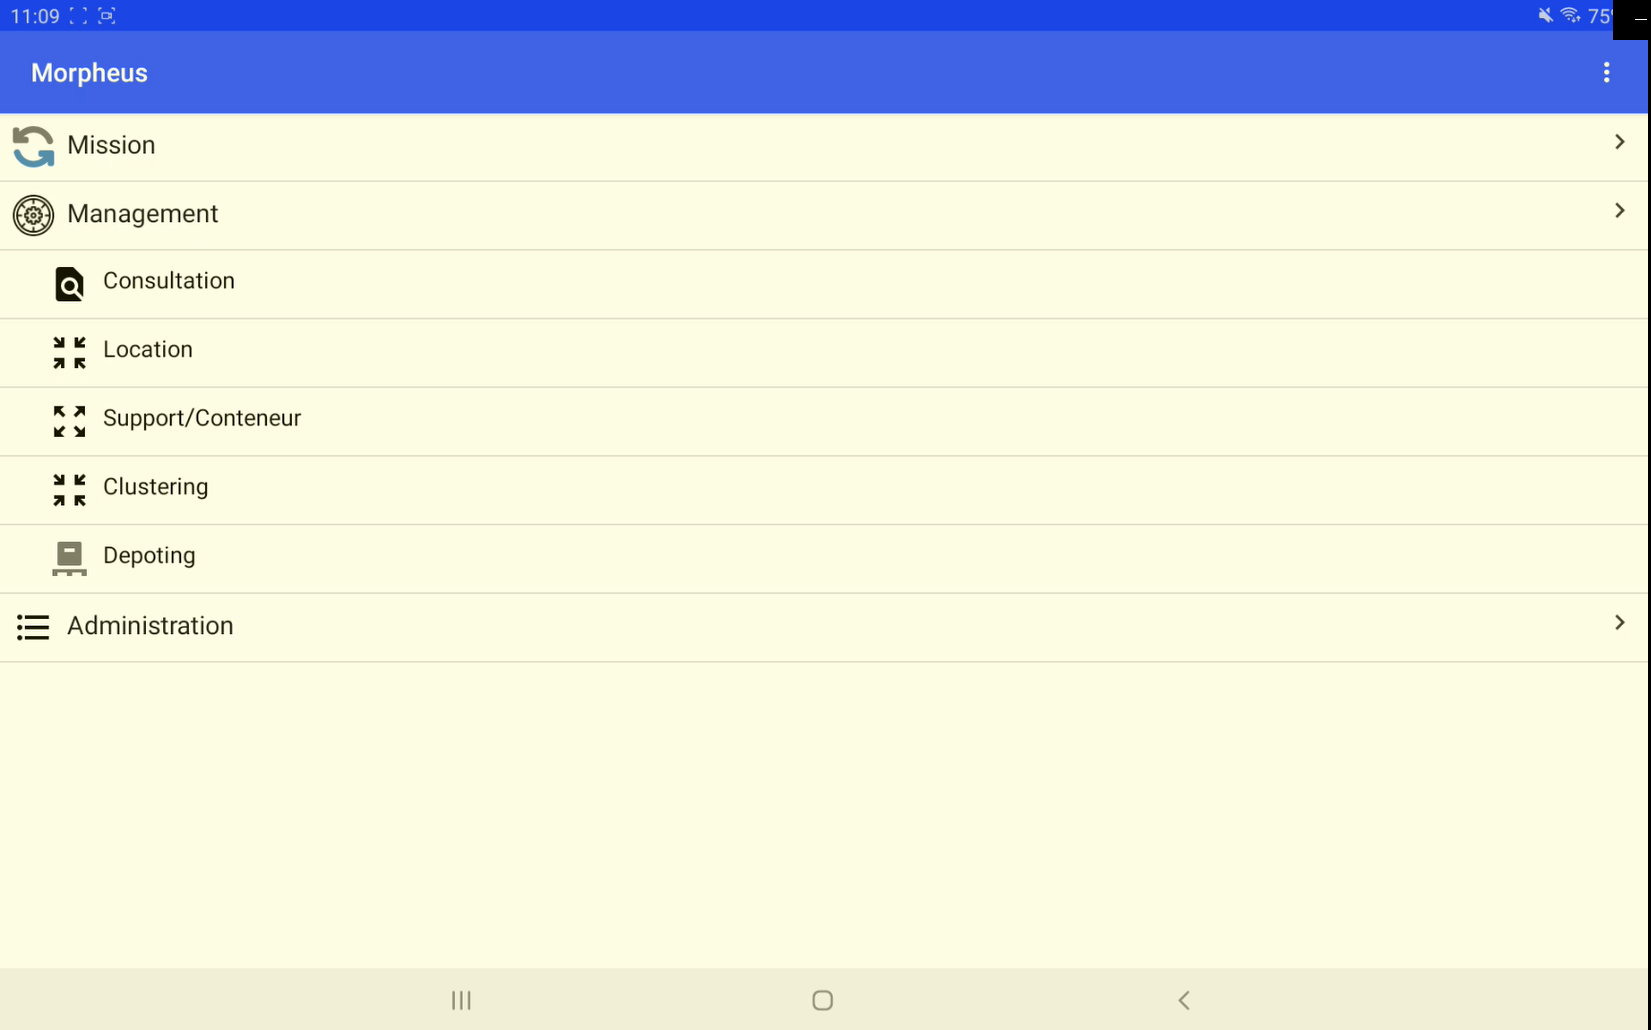
\includegraphics[width=0.7\linewidth]{application/user_menu_other_tab.PNG}
				\end{center}
				\caption{Écran du menu utilisateur de l'application}
				\label{fig:applications:user_menu_other_tab}
			\end{figure}	

			\vfill

			\begin{figure}[h!]
				\begin{center}
					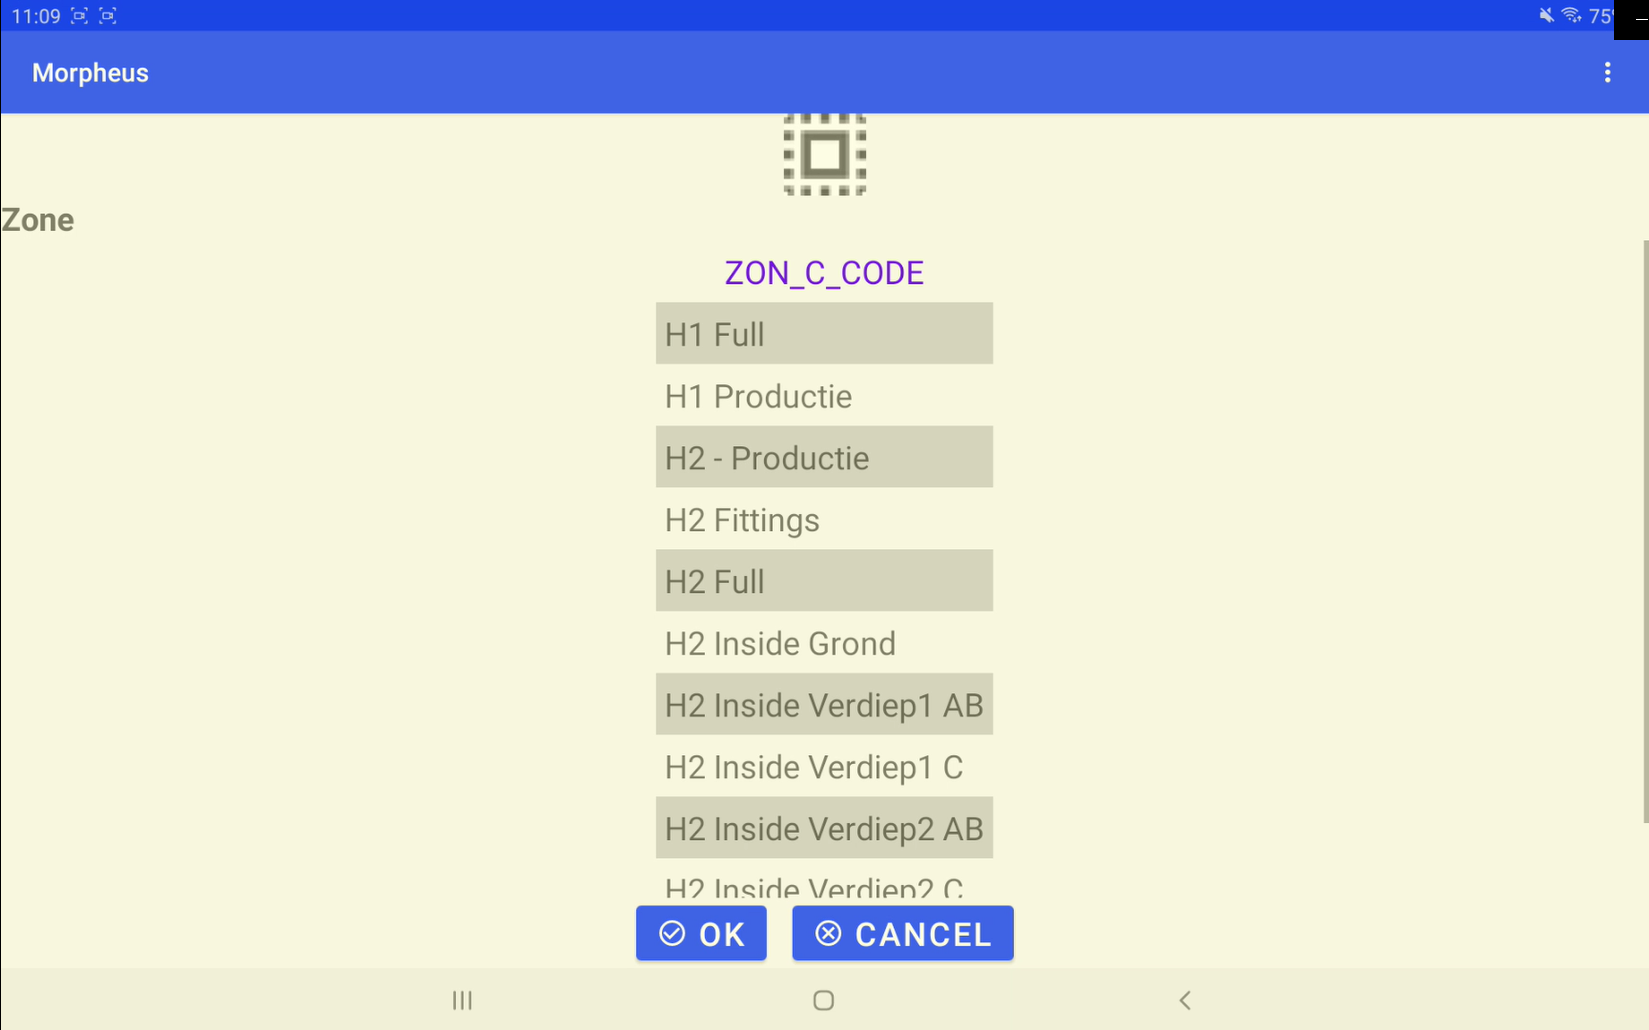
\includegraphics[width=0.7\linewidth]{application/zone.PNG}
				\end{center}
				\caption{Écran de sélection de la zone}
				\label{fig:applications:zone}
			\end{figure}	

		\newpage

	\phantomsection
	\section*{Résumés}
	\addcontentsline{toc}{section}{Résumés}
		\subsection*{Résumé}
		\addcontentsline{toc}{subsection}{Résumé}
	Pour résumer mon rapport de stage, je tiens à nouveau à remercier tous les acteurs qui ont pris part à la bonne réussite de mon stage. J'ai ainsi pu effectuer ce stage au sein de l'entreprise SSI SCHÄFER, pendant les mois de juillet et d'août 2022. L'entreprise SSI SCHÄFER est aujourd'hui l'un des premiers fournisseurs mondiaux de produits et systèmes logistiques pour le stockage, la préparation des commandes et la gestion des déchets. Ces solutions intralogistiques, partiellement ou entièrement automatisées, permettent d’optimiser les flux logistiques et l’aménagement des entrepôts et centres logistiques des clients, peu importe leur surface de stockage et leur secteur d’activité.\\

	Au cours de ce stage, j'ai intégré le service informatique en tant que stagiaire développeur et j'ai pu développer une application android, développée grâce à Android studio, afin de comparer cet outil de développement avec l'environnment Windev Mobile. Au cours de ce projet, j'ai principalement travaillé avec Monsieur Sébastien NICOD, qui lui a développé l'application actuelle, développée sous Windev Mobile. Pour m'aider j'ai aussi pu utiliser la documentation android qui est plutôt bien fournie. Pour conclure, ce stage est donc une très bonne réussite, que ce soit sur le plan professionnel ou humain et j'en suis très heureux.

		\subsection*{Summary}
		\addcontentsline{toc}{subsection}{Summary}
	To summarize my internship report, I would like to thank again all the actors who took part in the success of my internship. I was able to do this internship in the company SSI SCHÄFER, during the months of July and August 2022. SSI SCHÄFER is one of the world's leading suppliers of logistics products and systems for warehousing, order picking and waste management. These intralogistics solutions, partially or fully automated, allow to optimize the logistic flows and the layout of the warehouses and logistic centers of the customers, whatever their storage surface and their sector of activity.\\

	During this internship, I joined the IT department as an intern developer and I was able to develop an android application, developed with Android studio, in order to compare this development tool with the Windev Mobile environment. During this project, I mainly worked with Mister Sébastien NICOD, who developed the actual application, developed with Windev Mobile. To help me, I could also use the android documentation which is quite well provided. To conclude, this internship is a very good success, both professionally and humanly, and I am very happy.

		\subsection*{Zusammenfassung}
		\addcontentsline{toc}{subsection}{Zusammenfassung}
	Um meinen Praktikumsbericht zusammenzufassen, möchte ich mich noch einmal bei allen Beteiligten bedanken, die zum guten Gelingen meines Praktikums beigetragen haben. Ich habe mein Praktikum in den Monaten Juli und August 2022 bei der Firma SSI SCHÄFER absolvieren können. Das Unternehmen SSI SCHÄFER ist heute einer der weltweit führenden Anbieter von Logistikprodukten und -systemen für die Lagerung, Kommissionierung und das Abfallmanagement. Diese teilweise oder vollständig automatisierten intralogistischen Lösungen optimieren die logistischen Abläufe und die Einrichtung der Lagerhäuser und Logistikzentren der Kunden, unabhängig von der Lagerfläche und der Branche, in der sie tätig sind.\\
	
	Während dieses Praktikums trat ich als Entwicklungspraktikant in die IT-Abteilung ein und konnte eine Android-Anwendung entwickeln, die mithilfe von Android Studio entwickelt wurde, um dieses Entwicklungswerkzeug mit der Windev Mobile-Umgebung zu vergleichen. Während dieses Projekts arbeitete ich hauptsächlich mit Herrn Sébastien NICOD zusammen, der die aktuelle, unter Windev Mobile entwickelte Anwendung entwickelte. Um mir zu helfen, konnte ich auch die Android-Dokumentation nutzen, die ziemlich gut ausgestattet ist. Abschließend möchte ich sagen, dass dieses Praktikum sowohl auf beruflicher als auch auf menschlicher Ebene ein sehr guter Erfolg war und ich sehr glücklich darüber bin.
\end{document}